% -*- TeX:SI -*-
% slovene sub-mode for spell check

%\Large\textbf
\chapter[Direktni kinematični model]{Kinematični model robotskega 
manipulatorja \\ po metodologiji Denavit-Hartenberga in \\ metodi vektorskih parametrov}
%\chapter{Kinematični model robotskega manipulatorja po metodologiji Denavit-Hartenberga in metodi vektorskih parametrov}

\begin{mdframed}[backgroundcolor=green!20, shadow=true,roundcorner=8pt]
\vspace{-0.35cm}
\section{Cilji vaje}
\begin{itemize}
\item Uporaba znanja o računanju kinematike robotov pridobljenih na predavanjih,
\item utrjevanja znanja o računanju kinematike robotov pridobljenih na predavanjih s praktičnim preizkusom o pravilnosti rezultatov na pravih robotih,
\item postavljanje koordinatnih sistemov po DH metodi,
\item postavljanje koordinatnih sistemov po metodi z vektorskimi parametri,
\item spoznavanje razlik metod med pristopom DH in vektorskimi parametri,
\item preračun kinematičnega modela po obeh metodah za več različnih robotov,
\item preverjanje rezultata kinematike s pomočjo obeh metod ter izračuna kinematike krmilnika robota.

\end{itemize}
\end{mdframed}

\section{Naloga}

Po dveh metodah za izračun direktne kinematike, z metodo Denavit-Hartenbergovih (D-H) parametrov in metodo vektorskih parametrov, analitično izračunajte direktni
kinematični model za tri robotske manipulatorje.

\begin{description}

\item[Metoda Denavit-Hartenberga] \hfill \\ Za vsak sklep robotskega
manipulatorja podajte D-H parametre in izračunajte homogeno transformacijo za
preslikavo med koordinatnimi sistemi sklepov. Z množenjem $A_i$ matrik
izračunajte direktni kinematični model robotskega mehanizma v analitični
obliki. Za izbrano lego robota izračunajte tudi numerične vrednosti $T_6$
matrike. Za delo uporabite programski paket \emph{Mathematica}, pravilnost
rezultatov pa preverite s programskim paketom za vizualizacijo. V primeru
realnega robota rezultate preverite na robotskem krmilniku.

\item[Metoda vektorskih parametrov] \hfill \\
Z metodo vektorskih parametrov določite direktni geometrijski model
za robotske mehanizme. Glede na podano začetno konfiguracijo robota in podan referenčni koordinatni sistem, zapišite tabelo z vektorskimi parametri in jih uporabite za definiranje homogenih transformacijskih matrik med sklepi robota. Končni rezultat je homogena transformacijska matrika \textbf{T}, ki predstavlja produkt homogenih matrik in predstavlja geometrijski model robota oz. lego vrha robota glede na referenčni k.s. v odvisnosti od sklepnih spremenljivk. Pravilnost rezultata preverite s premikanjem sklepov realnega robota. Za delo uporabite programski paket Matlab z že pripravljeno predlogo in uporabniškim vmesnikom.

\end{description}

\section{Izvedba}

Homogene matrike služijo za opisovanje lege robotskega manipulatorja v 3D
prostoru. Pri zapisu direktnega kinematičnega modela si lahko pomagamo z D-H
notacijo ali metodo vektorskih parametrov. Ti predpisujeta, kako in kam je potrebno postaviti koordinatne sisteme
na manipulator, da je možno iz notranjih koordinat oz. zasukov v sklepih
določiti pozicijo in orientacijo vrha.

\subsection{Metoda Denavit-Hartenberga}

Glavna prednost \textbf{D-H notacije} je, da omogoča preslikavo med dvema koordinatnima sistemoma sklepov s samo štirimi
parametri.

\begin{mdframed}[backgroundcolor=green!20, shadow=false,roundcorner=12pt,topline
=false, rightline=false,bottomline=false,leftline=false]
\vspace{-0.35cm}

\vspace{4mm} \noindent \textbf{Pravila za postavitev koordinatnih
sistemov v sklepe robota}

\begin{enumerate}
\item\vspace*{-0.35cm} $0$-ti k.s. postavimo v os 1. sklepa. Ta k.s.
je fiksen in predstavlja bazni koordinatni sistem (WCS - World Coordinate
System) za reševanje kinematičnega modela. Os $z_0$ sovpada z osjo 1. sklepa.
Smer osi $x_0$ in $y_0$ je poljubna.

\item\vspace*{-0.35cm} Os $z_{i-1}$ leži v osi $i$-tega sklepa.


\item\vspace*{-0.35cm} Os $x_{i-1}$ je normalna na os $z_{i-1}$.
Orientacija je določena na tri možne načine:

\begin{enumerate}
\item\vspace*{-0.1cm} če sta osi sklepov $i-1$ in $i$ mimobežnici,
potem kaže os $x_{i-1}$ stran od osi sklepa $i-1$ v smeri najmanjše razdalje
med osema. Izhodišče k.s. $i-1$, ki leži na osi sklepa $i$, se nahaja v točki
povezave najkrajše razdalje med osema sklepov $i-1$ in $i$.

\item\vspace*{-0.1cm} če sta osi sklepov $i-1$ in $i$ vzporedni,
potem kaže $x_{i-1}$ stran od osi sklepa $i-1$.

\item\vspace*{-0.1cm} če se osi sklepov $i-1$ in $i$ sekata, potem
kaže $x_{i-1}$ v smeri vektorskega produkta \newline $z_{i-2}\times z_{i-1}$ .
Izhodišče koordinatnega sistema $i-1$ na osi sklepa $i$ se nahaja v presečišču
osi sklepov $i-1$ in $i$.

\item\vspace*{-0.1cm} os $y_{i-1}$ dopolnemo tako, da dobimo
desnosučni koordinatni sistem.
\end{enumerate}
\end{enumerate}

\end{mdframed}

\begin{figure}[h]
\centering
%\includegraphics[width=0.5\columnwidth]{denavit_hartenberg.eps}
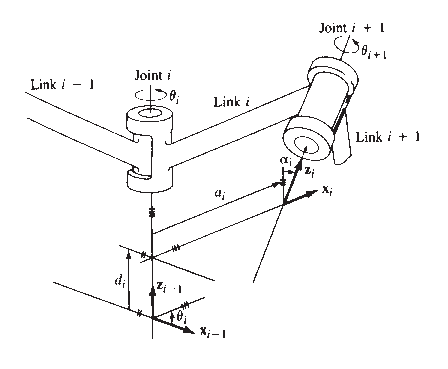
\includegraphics[width=0.75\columnwidth]{dh_bw.eps}
  \caption{\label{fig} Koordinatni sistemi v sklepih $i$ in $i+1$ po D-H notaciji}
\end{figure}

\begin{mdframed}[backgroundcolor=green!20, shadow=false,roundcorner=12pt,topline
=false, rightline=false,bottomline=false,leftline=false]
%\vspace{-0.35cm}

Prehod iz koordinatnega sistema $i-1$ v $i$ v posameznem sklepu opisuje
homogena transformacija $A_i$, ki je sestavljena iz zaporedja štirih operacij:
\begin{equation}\label{}
^{i-1}A_i = A_i = Rot(z,\theta_i)\;Trans(z,d_i)\;Trans(x,a_i)\;Rot(x,\alpha_i)
 \end{equation}

Zaporedje običajno bereme z leve proti desni, zato transformacije
izvajamo glede na trenutno lego koordinatnega sistema. Skupni
produkt transformacij je homogena matrika $A_i$:
\begin{equation}
A_i = \left[\begin{matrix} \cos \theta_i & -\cos \alpha_i \sin
\theta_i & \sin \alpha_i \sin \theta_i & a_i \cos \theta_i \cr \sin
\theta_i & \cos \alpha_i \cos \theta_i & -\cos \theta_i \sin \alpha_i
& a_i \sin \theta_i  \cr 0 & \sin \alpha_i & \cos \alpha_i & d_i \cr
0 & 0& 0 & 1 \end{matrix} \right]
\end{equation}

kjer je:

\begin{description}
\item \vspace*{-0.1cm} $\theta_i$ kot v sklepu med baznima vektorjema
$x_{i-1}$ in $x_{i}$ okoli $z_{i-1}$  v smislu pravila desne roke;

\item \vspace*{-0.1cm} $d_i$ razdalja med izhodiščem $i-1$
koordinatnega sistema do presečičča osi $y_{i-1}$ z $x_{i}$ vzdolž
$z_{i-1}$ osi;

\item \vspace*{-0.1cm} $a_i$ razdalja za premik vzdolž osi $x_{i}$
med sečiščem osi $z_{i-1}$ in $x_{i}$ do izhodišča koordinatnega
sistema $i$, to je najkrajša razdalja med osema $y_{i-1}$ in $x_{i}$;

\item \vspace*{-0.1cm} $\alpha_i$ kot zasuka od osi $z_{i-1}$ do osi
$z_{i}$ okoli $x_{i}$ z uporabo pravila desne roke.
\end{description}

Z upoštevanjem navedenih pravil je mogoče enostavno določiti homogene matrike
med posameznimi sklepi in s tem direktni kinematični model robotskega
mehanizma. Rezultat je tako imenovana matrika $T_6$. Matriko določimo kot
produkt posameznih homogenih matrik $A_i$:
\begin{equation}
T_6 = \prod_{i=1}^n A_i = A_1 \cdot A_2 \cdot A_3 \cdot A_4 \cdot A_5
\cdot A_6
\end{equation}

\end{mdframed}

\subsubsection{Programski paket Mathematica}

Programski paket \emph{Mathematica} je programsko orodje, ki omogoča
simbolično računanje. S pomočjo programskega paketa \emph{Mathematica} lahko
enostavno izračunamo direktni kinematični model v analitični ali numerični
obliki.

\vspace{5mm}

\noindent{\bf Osnovna pravila za delo s programom:}

\begin{itemize}
  \item Pisava enaka kot v matematiki. Realna števila nakažemo s piko.
Operatorji so:
\begin{verbatim}
^, -, +, /, ' ' ali *.
'3.5 x'  pomeni '3.5*x', a^2 je a a
\end{verbatim}

  \item Ločimo velike in male črke: 'a' ni isto kot 'A'.

  \item Matematične funkcije se začno z veliko začetnico. Argumente podamo v
oglatih oklepajih. Argumenti kotnih funkcij so v radianih.
\begin{verbatim}
Sin[2], Cos[ ], Log[ ], ArcTan[],
Exp[], Log[b,x], Abs[], Sqrt[]
\end{verbatim}

\item Znane matematične konstante so E, Pi, I za 2.718, 3.14, Sqrt[-1]

\item Grške črke pičemo po angleškem črkovanju: alpha, theta, mu

\item Vnos v tekstovnem uporabniškem vmesniku:
\begin{enumerate}
  \item \emph{Mathematica} čaka na vnos v obliki \\
   \verb@In[1]:=@
  \item Vtipkamo ukaz (\emph{italic}). Vnos potrdimo s hkratnim pritiskom tipk \newline \verb@Shift+Enter@ \\
 \verb@In[1]:=@ \emph{Sqrt[9]}
  \item Odgovor se glasi: \\
 \verb@Out[1]:=3@
\end{enumerate}

\item Pomoč o funckijah \emph{Mathematica} dobimo, če vtipkamo \verb@č@
\begin{description}
  \item[\emph{?Cos}] pove vse o tej funkciji
  \item[\emph{?C*}] seznam funkcij, ki se začno s črko C
\end{description}

\item Določanje spremenljivk:
\begin{verbatim}
    x = 3
    x = 3 a + 1
    x = "To je tekst"
\end{verbatim}

\item Brisanje spremenljivk:
\begin{verbatim}
    x = .
    Clear[x]
\end{verbatim}

\item Sklicevanje na rezultat i-tega vnosa:
\begin{verbatim}
    Out[5] = 0
    .
    .
    In[10]=x=Sqrt[%5] kvadratni koren od Out[5]
    Out[10]=Sqrt[10]
\end{verbatim}


\item \emph{Mathematica} rezultata ne izračuna, če to ni možno povsem precizno. K temu jo prisilimo z:
\begin{verbatim}
    In[11]=N[%]  samo % pomeni zadnji rezultat
    Out[11]=3.16228
\end{verbatim}

\item Oklepaji so štirih vrst:
\begin{description}
  \item[okrogli ()] za običajno grupiranje matematičnih izrazov
  \item[zaviti \{\}] za ponazoritev vektorjev, matrik: \verb@vekt1={1,2,0}@
  \item[dvojni oglati [[1]]] za indeksiraje komponent vektorjev
\end{description}

\item Računanje z matrikami in vektorji:
\begin{verbatim}
vektor= {x,y,z} matrika={{1,2},{3,4}} element=matrika[[1,2]]
vrsticni_vektor=matrika[[2]] :rezultat {3,4}
stolpicni_vektor=Transpose[matrika][[2]] :rez {2,5}
mat=matrika.matrika  :mnozenje matrik
trans_mat=Transpose[matrika] :transponirano
inv_mat=Inverse[matrika] :inverzna matrika
\end{verbatim}

\item Vključitev dodatnih paketov:
\begin{verbatim}
    Needs["Algebra`Trigonometry`"]
    Needs["Geometry`Robotics`"]
    Needs["Calculus`VectorAnalysis`"]
\end{verbatim}


\item Shranjevanje rezultatov in definicij v datoteko:
\begin{verbatim}
    Save "file", f1, f2, f3
\end{verbatim}

\item Funkcija za izračun homogene matrike $A_i$:
\begin{verbatim}
    A1 = HDHMatrix[theta1, d1, a1, alpha1]
\end{verbatim}
Funkcija $HDHMatrix$ je del dodatnega paketa $Robotics$.

\end{itemize}

\clearpage
\subsubsection{Programski paket za vizualizacijo robotskega mehanizma RoboAnalyzer}

Programski paket RoboAnalyzer je namenjen vizualizaciji robotskega mehanizma, ki ga definiramo s tabelo Denavit-Hartenbergovih parametrov. Namenjen je za poučevanje direktne kinematike, inverzne kinematike in dinamike robotov. Program vključuje določitev kinematičnega modela robota s pomočjo Denavit-Hartenbergove notacije, preprosto vizualizacijo robota z koordinatnimi sistemi sklepov in izračun transformacijskih matrik glede na vpisane parametre. Programski paket RoboAnalyzer je na voljo na spletni strani \texttt{http://www.roboanalyzer.com/}. Na spletni strani se nahajajo tudi natančna navodila za uporabo programa.


Program zaženete z zagonsko datoteko \texttt{RoboAnalyzer.exe}. Odpre se glavno okno programa. V podoknu D-H Parameters izberete število prostostnih stopenj robota, konfiguracijo robota, ter vpišete vse potrebne D-H parametre.



\begin{figure}[h]
	\centering 
	\psfrag{st}[c][c][0.8][0]{št. prost. stopenj robota}
	\psfrag{kon}[Bl][l][0.8][0]{konfiguracija robota}
	\psfrag{pard}[Bl][l][1.0][0]{$d_i$}	
	\psfrag{parthof}[Bl][l][1.0][0]{$\theta_i$}
	\psfrag{paraa}[Bl][l][1.0][0]{$a_i$}		
	\psfrag{paral}[Bl][l][1.0][0]{$\alpha_i$}		
	\psfrag{parth1}[Bl][l][0.8][0]{za\v cetna $\theta_i$}		
	\psfrag{parth2}[Bl][l][0.8][0]{kon\v cna $\theta_i$}		
	\psfrag{nko}[Bl][l][0.8][0]{ustvarjanje novega robota}
	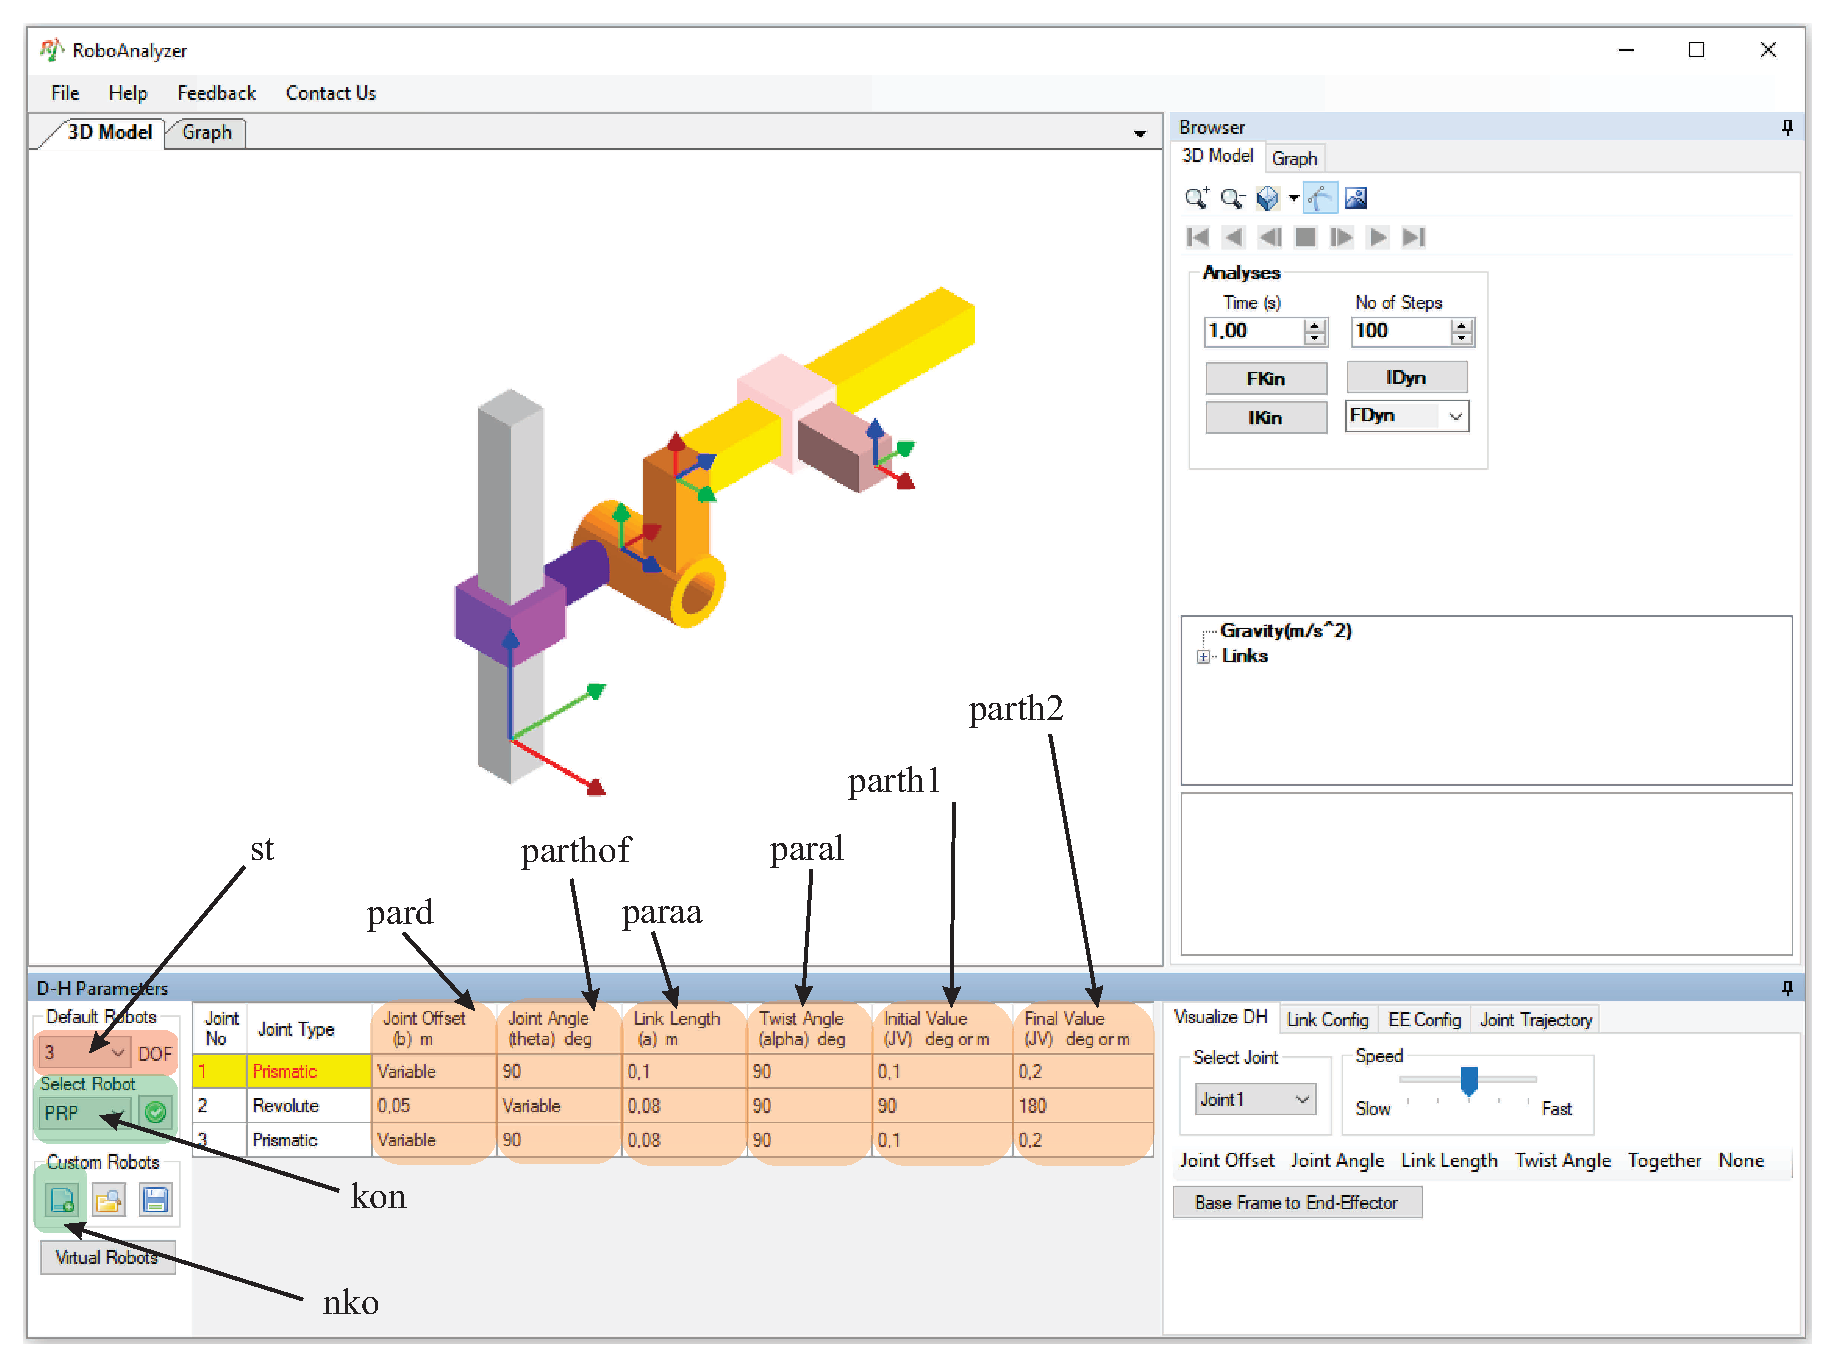
\includegraphics[width=0.85\columnwidth]{RA1.eps}
	\caption{\label{RA1} Okno programskega paketa RoboAnalyzer.}
\end{figure}



V oknu \verb@D-H Parameters@ lahko izberete \v ze ustvarjene konfiguracije v podoknu \verb@Default Robots@. Na začetku izberete število prostostnih stopenj, ki jih ima robot, ter konfiguracijo robota (razporeditev rotacijskih in translacijskih sklepov). \v Ce v \verb@Default Robots@ ni \v zelene konfiguracije robota, kot je to v primeru Stanford robota, potem ustvarite novega robota z ikono \verb@Add New Robot@ v podoknu \verb@Custom Robots@.

Naslednji korak je, da vpišete D-H parametre:

\begin{description}
	\item[Parameter $d_i$:] Joint Offset (b) mm.
	\item[Parameter $\theta_i$:] Joint Angle (theta) deg.
	\item[Parameter $a_i$:] Link Length (a) mm.
	\item[Parameter $\alpha_i$:] Twist Angle (alpha) deg.
	\item[Začetna vrednost parametra sklepa:] Intial Value (JV) deg or mm.
	\item[Končna vrednost parametra sklepa:] Final Value (JV) deg or mm.	
\end{description}


\subsection{Direktni geometrijski model robota z vektorskimi parametri}

\vspace{0.2cm}
Za zapis \textbf{direktnega geometrijskega modela}, ki predstavlja
lego vrha robota glede na njegov referenčni koordinatni
sistem lahko uporabimo metodo z vektorskimi parametri.
\\
\\
\begin{mdframed}[backgroundcolor=green!20, shadow=false,roundcorner=12pt,topline
=false, rightline=false,bottomline=false,leftline=false]

\textbf{Postopek določanja vektorskih parametrov}

\begin{enumerate}
    \item \vspace*{-0.35cm} Mehanizem postavimo v začetno lego,
    kjer  so vrednosti sklepnih koordinat enake nič ($\vartheta_i$ =
    0, $d_i$ = 0, i = 1, 2, ...,n). Pri tem morajo biti osi sklepov
    vzporedne osem referenčnega koordinatnega sistema $x_0, y_0, z_0$.
    \\
    \emph{Vsi roboti so \v ze narisani v referenčnih legah. V teh
    legah imajo tudi realni roboti vrednosti notranjih spremenljivk enake $0$.}    \\%
\vspace{-0.4cm}
    \item V središče sklepa $i$ namestimo lokalne
    koordinatne sisteme $x_i, y_i, z_i$. Njihove osi so vzporedne osem referenčnega k.s. $x_0, y_0,
    z_0$.
    \\
    \emph{Pri vaji so, na prilo\v zenih skicah robotov, izhodišča lokalnih
    koordinatnih sistemov označena.}\\%
\vspace{-0.4cm}
    \item V vsako os mehanizma $i = 1, 2, ..., n$
    postavimo enotski sklepni \mbox{vektor $\textbf{e}_i$.} Njegova smer
    kaže v smeri ene osi koordinatnega sistema $x_i, y_i, z_i$. V
    smeri tega vektorja merimo pozitivno translacijsko koordinato $d_i$,
    okrog njega (obratna smer urinega kazalca) pa pozitivno rotacijsko
    \mbox{koordinato $\vartheta_i$.} \\%
\vspace{-0.4cm}
    \item Med izhodišči lokalnih koordinatnih
    sistemov povlečemo segmentne vektorje $\textbf{b}_{i-1}$.
    Segmentni vektor $\textbf{b}_n$ leži med izhodiščem
    koordinatnega sistema $x_n, y_n, z_n$ in referenčno točko na
    vrhu mehanizma.%
\end{enumerate}
\vspace{0.2cm} %
\textbf{Homogene transformacijske matrike določimo s spodnjo
predlogo:}

\begin{equation*}
    \textbf{H}_\textbf{{i-1,i}} =
    \begin{bmatrix}
     & \textbf{Rot}_{i-1,i} &  & d_i\textbf{e}_{i}^{i-1}+\textbf{b}_{i-1,i}^{i-1} \\%
    0              &   0                &    0  &   1     \\%
    \end{bmatrix}
\end{equation*}
\vspace{-0.2cm}

\end{mdframed}

V določenih primerih vpeljemo \v se dodatni koordinatni sistem v vrh
robota oz. v referenčno točko prijemala. Označimo ga z $x_{n+1},
y_{n+1}, z_{n+1}$. Med koordinatnim sistemom $x_{n}, y_{n}, z_{n}$
in $x_{n+1}, y_{n+1}, z_{n+1}$ ni nobenih prostostnih stopenj, saj
sta oba pripeta na isti segment, zato je
transformacija konstantna. \\
\textbf{\emph{\v Ce hočemo primerjati rezultat lege vrha dejanskega
robota, kot recimo robot Epson PS3 ali Motoman MH5, z na\v sim modelom, je vpeljava dodatnega k.s. oz.
dodatne transformacije na vrh robota nujna, saj se drugače
orientacija vrha robota v našem modelu ne ujema z orientacijo
koordinatnega sistema na vrhu realnega robota. }} \vspace{0.2cm}



\section{Domača naloga in uvodni del}

\paragraph{Domača naloga}
Za robot Stanford za domačo nalogo glede na sliko robota (Slika 1) zapišite ustrezno Denavit-Hartenbergovo tabelo z ustreznimi DH parametri.

Poleg robota Stanford isto naredite tudi za robot Adept SCARA. Vendar pa pri tem robotu kinematični model, poleg DH metode, zapišite tudi po metodi z vektorskimi parametri. Tudi pri tej metodi na sliko (Slika 2) narišite potrebne koordinatne sisteme in vektorje ter zapišite tabelo vektorskih parametrov.

\paragraph{Pripravljalni termin}
Pripravljalni termin je namenjen preverjanju pravilnosti za domačo nalogo zapisanega kinematičnega modela robotov Standford in Adept SCARA. Preverjanje za robot Standford bo potekalo v okolju RoboAnalyzer in v okolju Mathematica, za robot Adept SCARA pa v okolju RoboAnalyzer in v okolju Matlab.


\subsection{Naloga 1: Direktni kinematični model za robota Adept One}\label{scara}

Robot Adept One je robot SCARA konfiguracije s štirimi prostostnimi stopnjami.
Na sliki \ref{scara} je predstavljen SCARA robot s tremi rotacijskimi in enim
translacijskim sklepom.

%\begin{figure}[h]
%\centering \psfrag{a1}[Bl][l][1.5][0]{$a_1$}
%\psfrag{a2}[Bl][l][1.5][0]{$a_2$}
%\psfrag{d1}[Bl][l][1.5][0]{$d_1$}
%\psfrag{d3}[Bl][l][1.5][0]{$d_3$}
%\psfrag{d4}[Bl][l][1.5][0]{$d_4$}
%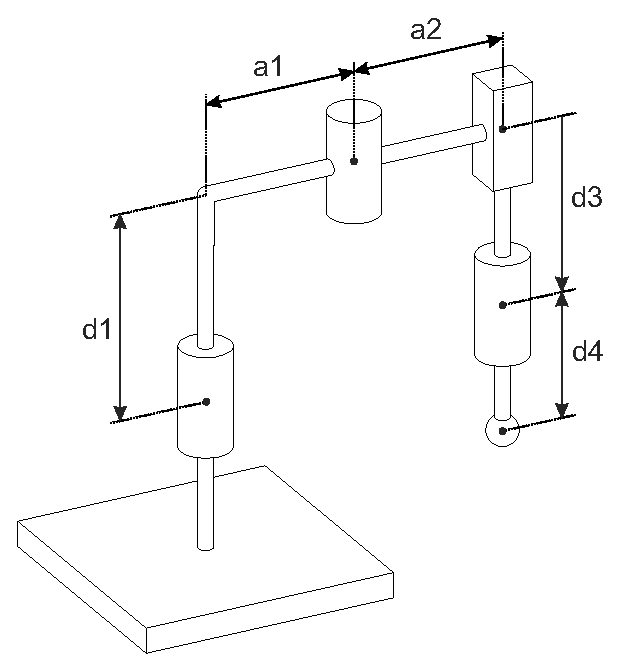
\includegraphics[width=0.6\columnwidth]{scara3.eps}
%  \caption{\label{scara} Robot SCARA konfiguracije s štirimi DOF}
%\end{figure}

\begin{figure}[h]
\centering \psfrag{a1}[Bl][l][1.5][0]{$a_1$}
\psfrag{a2}[Bl][l][1.5][0]{$a_2$}
\psfrag{d1}[Bl][l][1.5][0]{$d_1$}
\psfrag{d3}[Bl][l][1.5][0]{$d_3$}
\psfrag{d4}[Bl][l][1.5][0]{$d_4$}
\psfrag{x0}[Bl][l][1.5][0]{$x_0$}
\psfrag{z0}[Bl][l][1.5][0]{$z_0$}
\psfrag{y0}[Bl][l][1.5][0]{$y_0$}
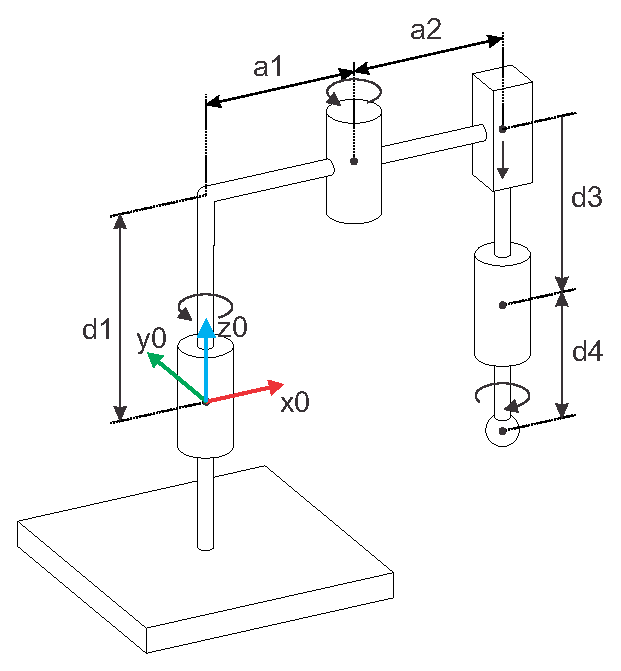
\includegraphics[width=0.6\columnwidth]{scara3VektorskiParametri.eps}
  \caption{\label{scara} Robot SCARA konfiguracije s štirimi DOF}
\end{figure}

\subsubsection{Metoda Denavit-Hartenberga}

Z upoštevanjem D-H pravil označite koordinatne sisteme in določite D-H parametre.
Doma vrišite koordinatne sisteme in pripravite DH tabelo.



Izračunajte tudi numerično vrednost matrike $T_4$, če so podani naslednji
kinematični parametri:
\begin{eqnarray}
d_1 &=& 437 \; mm \nonumber \\
d_2 &=& 200 \; mm \nonumber \\
a_1 &=& 425 \; mm \nonumber \\
a_2 &=& 375 \; mm \nonumber \\
%\nonumber \\
%\theta_1 &=& 0 \; rd = 0 č \nonumber \\
%\theta_2 &=& 0 \; rd = 0 č \nonumber \\
%d_3 &=& 0 \; mm \nonumber \\
%\theta_4 &=& 0 \; rd = 0 č \nonumber
\end{eqnarray}

Navedene vrednosti uporabite tudi pri načrtovanju modela robota v programu
RoboAnalyzer.  Za končno stanje spremenljivk v sklepih
$(\theta_1, \theta_2, d_3$ in $\theta_4)$ uporabite vrednost $0$. Opazujte
premike posameznih sklepov. Pazite tudi na pravilno orientacijo prijemala
pritrjenega na vrh modela robotskega manipulatorja.

\subsubsection{Metoda vektorskih parametrov}

V ukazni vrstici okolja Matlab se vpiše:\\
\vspace{-0.4cm}\\%
\textbf{open Za$\_$studente$\_$SCARA}  \\ %
\vspace{-0.4cm}\\%

% ********************************************************************

\begin{mdframed}[backgroundcolor=green!20, shadow=false,roundcorner=12pt,topline
=false, rightline=false,bottomline=false,leftline=false]
        \vspace{0.2cm}
Z upoštevanjem navodil za postavljanje vektorskih parametrov
postavite ustrezno koordinatne sisteme, sestavite tabelo z
vektorskimi parametri in na podlagi le te definirajte direktni
geometrijski model robota. V nadaljevanju definirajte homogene
transformacijske matrike \textbf{H}$_\textbf{01}$,
\textbf{H}$_\textbf{12}$, \textbf{H}$_\textbf{23}$,
\textbf{H}$_\textbf{34}$ in \textbf{T}. Definirajte jih z če
pripravljenimi funkcijami \emph{H$\_$RotX$\_$Trans},
\emph{H$\_$RotY$\_$Trans} in \emph{H$\_$RotZ$\_$Trans}. Po
definiranju vseh štirih \textbf{H} matrik z ustreznim zaporedjem
množenja izračunajte matriko \textbf{T}, ki predstavlja lego vrha
robota (zadnji koordinatni sistem) glede na referenčni koordinatni
sistem.
\end{mdframed}

%\vspace{-0.5cm}

\begin{mdframed}[backgroundcolor=blue!20, shadow=false,roundcorner=12pt,topline
=false, rightline=false,bottomline=false,leftline=false]
        \vspace{0.2cm}
\textbf{Primer definiranja matrike H01:}\\
Koordinatni sistem v sklepu 1 je zarotiran po osi \emph{z} za
$\phi$, transliran po \emph{x} za p$_1$, po \emph{y} za 0 in po
\emph{z} za p$_3$, vse glede na prejšnji koordinatni sistem.
Funkcijo, s katero zapišemo lego koordinatnega sistema 1 glede na
prejšnji koordinatni sistem 0, zapišemo:\vspace{0.2cm}\\%
\vspace{0.2cm}%
\hspace*{3.5cm}\textbf{H01 = H$\_$RotZ$\_$Trans($\phi$, p$_1$, 0,
p$_3$);}
        \vspace{0.0cm}
    \end{mdframed}

% ********************************************************************

\vspace{0.2cm}%
Spodaj je prikazana predloga \emph{Za$\_$studente$\_$SCARA.m} za
pisanje programa za izračun direktnega kinematičnega modela za robot
Epson E2S651 (SCARA). Vpisuje se samo vrstice, ki so označene s
\emph{$\%$ STUDENT}. Vhodni parametri funkcije so: $h_1$, $h_2$,
$h_3$, $l_1$, $l_2$, $th_1$, $th_2$, $d_3$ in $th_4$. Te uporabite v
kombinaciji s funkcijami za zapis homogenih transformacijskih
matrik.


\begin{figure}[h]
\scriptsize%
\textcolor[rgb]{0.13,0.55,0.13}{\textbf{\texttt{$\%$ ************************************}}}\\ %
\textcolor[rgb]{0.13,0.55,0.13}{\textbf{\texttt{$\%$ *** PREDLOGA ZA PISANJE PROGRAMA ***}}}\\ %
\textcolor[rgb]{0.13,0.55,0.13}{\textbf{\texttt{$\%$ ************************************}}}\\ %
\textcolor[rgb]{0.13,0.55,0.13}{\textbf{\texttt{$\%$ Programske vrstice vpisujete le v področja, ki so označena s STUDENT!}}}\\ %
\textcolor[rgb]{0.13,0.55,0.13}{\textbf{\texttt{$\%$ Ostale vrstice pustite nedotaknjene}}}\\ %
\textcolor[rgb]{0.13,0.55,0.13}{\textbf{\texttt{$\%$ *************************************************************************}}}\\ %
\textcolor[rgb]{0.00,0.00,0.00}{\textbf{\texttt{$\%$ function Za$\_$studente$\_$SCARA(h1,h2,h3,l1,l2,th1,th2,d3,th4)}}}\\ %
\\ %
\textcolor[rgb]{0.13,0.55,0.13}{\textbf{\texttt{$\%$ *}}}\\ %
\textcolor[rgb]{0.13,0.55,0.13}{\textbf{\texttt{$\%$ **}}}\\ %
\textcolor[rgb]{0.13,0.55,0.13}{\textbf{\texttt{$\%$ ***}}}\\ %
\textcolor[rgb]{0.13,0.55,0.13}{\textbf{\texttt{$\%$ ***************************}}}\\ %
\textcolor[rgb]{0.13,0.55,0.13}{\textbf{\texttt{$\%$ *** VRSTICE ZA STUDENTE ***}}}\\ %
\textcolor[rgb]{0.13,0.55,0.13}{\textbf{\texttt{$\%$ *************************************************************************}}}\\ %
\textcolor[rgb]{0.13,0.55,0.13}{\textbf{\texttt{$\%$ Definiranje homogenih transformacijskih matrik med sklepi}}}\\ %
\textbf{\texttt{\hspace*{1cm}H01 = \textcolor[rgb]{0.13,0.55,0.13}{$\%$ STUDENT}}}\\ %
\textbf{\texttt{\hspace*{1cm}H12 = \textcolor[rgb]{0.13,0.55,0.13}{$\%$ STUDENT}}}\\ %
\textbf{\texttt{\hspace*{1cm}H23 = \textcolor[rgb]{0.13,0.55,0.13}{$\%$ STUDENT}}}\\ %
\textbf{\texttt{\hspace*{1cm}H34 = \textcolor[rgb]{0.13,0.55,0.13}{$\%$ STUDENT}}}\\ %
\\ %
\textcolor[rgb]{0.13,0.55,0.13}{\textbf{\texttt{$\%$ Multiplikacija homogenih transformacijskih matrik za izračun}}}\\ %
\textcolor[rgb]{0.13,0.55,0.13}{\textbf{\texttt{$\%$ geometrijskega modela robota}}}\\ %
\textbf{\texttt{\hspace*{1cm}T = \textcolor[rgb]{0.13,0.55,0.13}{$\%$ STUDENT}}}\\ %
\textcolor[rgb]{0.13,0.55,0.13}{\textbf{\texttt{$\%$ *************************************************************************}}}\\ %
\textcolor[rgb]{0.13,0.55,0.13}{\textbf{\texttt{$\%$ ***}}}\\ %
\textcolor[rgb]{0.13,0.55,0.13}{\textbf{\texttt{$\%$ **}}}\\ %
\textcolor[rgb]{0.13,0.55,0.13}{\textbf{\texttt{$\%$ *}}}\\ %

\end{figure}

% ********************************************************************

\begin{mdframed}[backgroundcolor=green!20, shadow=false,roundcorner=12pt,topline
=false, rightline=false,bottomline=false,leftline=false]
        \vspace{0.2cm}
Ob upoštevanju navodil za postavljanje vektorskih parametrov,
postavite ustrezno koordinatne sisteme, sestavite tabelo z
vektorskimi parametri in na podlagi teh parametrov definirajte
direktni kinematični model. V nadaljevanju definirajte homogene
transformacijske matrike \textbf{H}$_\textbf{01}$,
\textbf{H}$_\textbf{12}$, \textbf{H}$_\textbf{23}$,
\textbf{H}$_\textbf{34}$, \textbf{H}$_\textbf{45}$,
\textbf{H}$_\textbf{56}$, \textbf{H}$_\textbf{67}$ in \textbf{T}. Za
definiranje matrike \textbf{H}$_\textbf{67}$ si pomagajte s sliko
\ref{fShemaPS3}.  Matrike \textbf{H} definirajte z če pripravljenimi
funkcijami \emph{H$\_$RotX$\_$Trans}, \emph{H$\_$RotY$\_$Trans} in
\emph{H$\_$RotZ$\_$Trans}. Po definiranju vseh sedmih \textbf{H}
matrik z ustreznim zaporedjem množenja izračunajte matriko
\textbf{T}, ki predstavlja lego vrha robota (zadnji koordinatni
sistem) glede na referenčni koordinatni sistem. \vspace{0.2cm}
\end{mdframed}

Ko zapišemo vse vrstice v obeh datotekah, začenemo
uporabniško okno za preverjanje rezultatov. V ukazno vrstico programskega okolja Matlab vpišemo\\
\vspace{-0.2cm}\\%
\textbf{RezultatiGUI} \\ %
\vspace{-0.2cm}\\%
in odpre se okno s slike \ref{fGUI}.

\begin{figure}[h]
    \centering
    \includegraphics[width=0.74\textwidth]{07_GUI_Scara.eps}
    \vspace{0.2cm}
%    \\%
%    \includegraphics[width=0.74\textwidth]{07_GUI_PS3.eps}
%    \vspace{-0.3cm}
    \caption{uporabniški vmesnik za preverjanje rezultatov}
    \label{fGUI}
\end{figure}

Objekti v uporabniškem vmesniku:

\begin{enumerate}
    \vspace{-0.2cm}%
    \item[] \textbf{Izberite} $\longrightarrow$ Robot, za katerega bomo preverjali kinematični model! %
    \vspace{-0.2cm}%
    \item[] \textbf{Sklepne sprem.} $\longrightarrow$ Vpisujemo vrednosti sklepnih spremenljivk. %
    \vspace{-0.2cm}%
    \item[] \textbf{Matrika T} $\longrightarrow$ Transformacijska matrika vrha robota glede na ref. k.s. %
    \vspace{-0.2cm}%
    \item[] \textbf{Vaša izračunana lega} $\longrightarrow$ Pozicija in orientacija vrha glede na ref. k.s. %
    \vspace{-0.2cm}%
    \item[] \textbf{Izračun modela robota z vektorskimi parametri} $\longrightarrow$ Izračunamo kinematični model s svojimi parametri! %
\end{enumerate}

Na sliki je robot izrisan v legi, ko so
vrednosti notranjih spremenljivk enake 0. Pogled na sliki je s
sprednje strani prvega segmenta, kar označuje položaj ploščice na
prvem segmentu. Narisane so tudi pozitivne smeri rotacije in
translacije na robotu.



% ********************************************************************
\begin{mdframed}[backgroundcolor=green!20, shadow=false,roundcorner=12pt,topline
=false, rightline=false,bottomline=false,leftline=false]
Pravilnost direktnega kinematičnega modela preverite z vpisovanjem
ustreznih vrednosti notranjih spremenljivk v Matlab uporabniški
vmesnik z imenom \emph{RezultatiGUI}. \textbf{V uporabniškem
vmesniku mora biti izbran robot Robot SCARA (4 DOF)}. S klikom na
gumb \emph{Izračun modela robota z vektorskimi parametri} izračunate
polja \emph{"Matrika T"} in \emph{"Vaša izračunana lega"}. Testne
vrednosti notranjih spremenljivk in rezultati so podani na slikah
\ref{fRezultatiScara}.
\end{mdframed}

% ********************************************************************

\begin{figure}[!h]
    \centering
    \includegraphics[width=0.82\textwidth]{02_SCARA_Test1.eps}\vspace{0.1cm}\\%
\end{figure}

\begin{figure}[!h]
    \centering
    \includegraphics[width=0.82\textwidth]{02_SCARA_Test2.eps}\vspace{0.1cm}\\%
\end{figure}

\begin{figure}[!h]
    \centering
    \includegraphics[width=0.82\textwidth]{02_SCARA_Test3.eps}\\%
    \vspace{-0.3cm}
    \caption{Vrednosti notranjih spremenljivk in rezultati za robot Epson E2S651}
    \label{fRezultatiScara}
\end{figure}


\newpage


\subsection{Naloga 2: Direktni kinematični model za robot Stanford}\label{stanford}

Robot Stanford je robot antropomorfne konfiguracije s šestimi prostostnimi
stopnjami gibanja, ki vključujejo pet rotacijskih sklepov in enega
translacijskega. Robot je predstavljen na sliki \ref{stanford}.
\begin{figure}[h]
\centering \psfrag{o}[Bl][l][1.0][0]{$O$} \psfrag{x0}[Bl][l][1.0][0]{$x_0$}
\psfrag{y0}[Bl][l][1.0][0]{$y_0$} \psfrag{z0}[Bl][l][1.0][0]{$z_0$}
\psfrag{x1}[Bl][l][1.0][0]{$x_1$} \psfrag{y1}[Bl][l][1.0][0]{$y_1$}
\psfrag{z1}[Bl][l][1.0][0]{$z_1$} \psfrag{x2}[Bl][l][1.0][0]{$x_2$}
\psfrag{y2}[Bl][l][1.0][0]{$y_2$} \psfrag{z2}[Bl][l][1.0][0]{$z_2$}
\psfrag{x3}[Bl][l][1.0][0]{$x_3$} \psfrag{y3}[Bl][l][1.0][0]{$y_3$}
\psfrag{z3}[Bl][l][1.0][0]{$z_3$} \psfrag{x4}[Bl][l][1.0][0]{$x_4$}
\psfrag{y4}[Bl][l][1.0][0]{$y_4$} \psfrag{z4}[Bl][l][1.0][0]{$z_4$}
\psfrag{x5}[Bl][l][1.0][0]{$x_5$} \psfrag{y5}[Bl][l][1.0][0]{$y_5$}
\psfrag{z5}[Bl][l][1.0][0]{$z_5$} \psfrag{x6}[Bl][l][1.0][0]{$x_6$}
\psfrag{y6}[Bl][l][1.0][0]{$y_6$} \psfrag{z6}[Bl][l][1.0][0]{$z_6$}
\psfrag{d1}[Bl][l][1.0][0]{$d_1$} \psfrag{d2}[Bl][l][1.0][0]{$d_2$}
\psfrag{d3}[Bl][l][1.0][0]{$d_3$} \psfrag{d6}[Bl][l][1.0][0]{$d_6$}
\psfrag{th1}[Bl][l][1.0][0]{$\theta_1$}
\psfrag{th2}[Bl][l][1.0][0]{$\theta_2$}
\psfrag{th4}[Bl][l][1.0][0]{$\theta_4$}
\psfrag{th5}[Bl][l][1.0][0]{$\theta_5$}
\psfrag{th6}[Bl][l][1.0][0]{$\theta_6$} \psfrag{OC}[Bl][l][1.0][0]{izhodišča
se ujemajo} \psfrag{d4d5}[Bl][l][1.0][0]{$d_4 = d_5 = 0$}
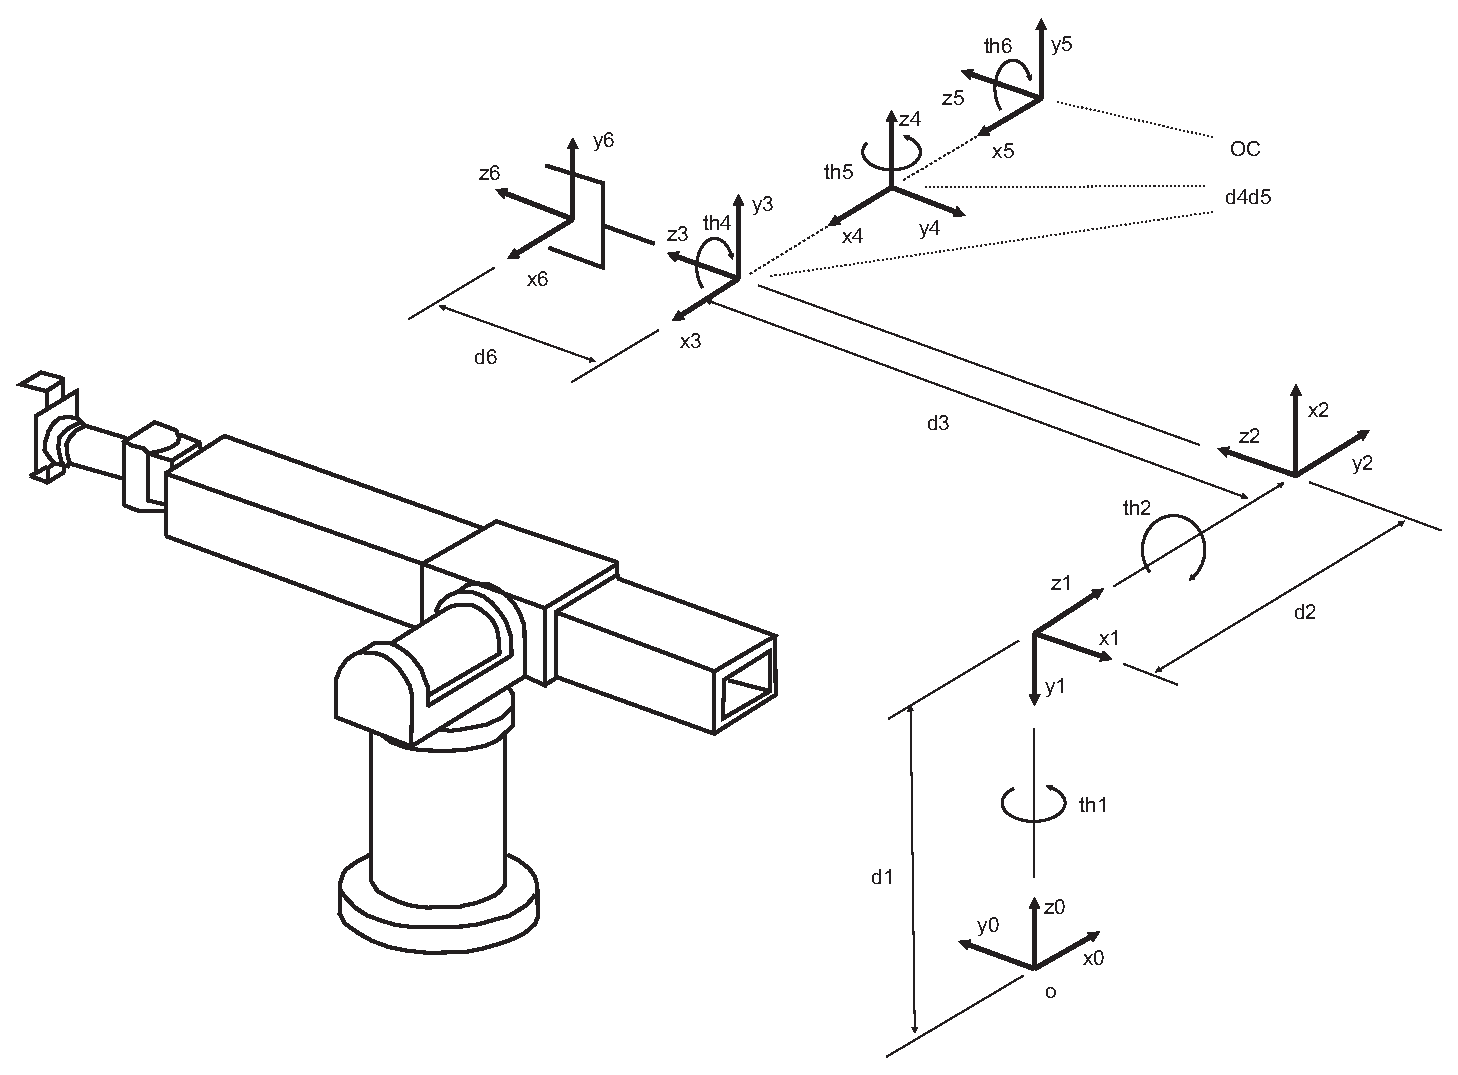
\includegraphics[width=0.85\columnwidth]{stanford_2.eps}
  \caption{\label{stanford} Robot Stanford s šestimi DOF}
\end{figure}

V laboratoriju s pomočjo programskega paketa \emph{Mathematica} najprej izračunajte
transformacijske matrike $A_i$ med posameznimi sklepi (npr.: matrika $A_{01}$
- transformacijska matrika med 0. KS in 1. KS,...). Direktno kinematiko robota
izračunajte kot matriko $T_6$ s pomočju množenja posameznih $A_i$ matrik. Pripravljena je
predloga \emph{Mathematica} datoteke za stanford robota, odprite datoteko \verb"stanford.nb":

\small %
\texttt{} \\
\texttt{Needs["Geometry`Robotics`"];} \\
\texttt{} \\
\texttt{d1 = \#;} \\
\texttt{d2 = \#;} \\
\texttt{d3 = \#;} \\
\texttt{d6 = \#;} \\
\texttt{A01 = HDHMatrix[\#, \#, \#, \#];} \\
\texttt{A12 = HDHMatrix[\#, \#, \#, \#];} \\
\texttt{A23 = HDHMatrix[\#, \#, \#, \#];} \\
\texttt{A34 = HDHMatrix[\#, \#, \#, \#];} \\
\texttt{A45 = HDHMatrix[\#, \#, \#, \#];} \\
\texttt{A56 = HDHMatrix[\#, \#, \#, \#];} \\
\texttt{T6 = \#.\#.\#.\#.\#.\#;} \\
\texttt{} \\
\texttt{A01 // MatrixForm} \\
\texttt{A12 // MatrixForm} \\
\texttt{A23 // MatrixForm} \\
\texttt{A34 // MatrixForm} \\
\texttt{A45 // MatrixForm} \\
\texttt{A56 // MatrixForm} \\
\texttt{Simplify[T6] // MatrixForm} \\
\texttt{} \\
\texttt{th1 = \#} $^{\circ}$; \\
\texttt{th2 = \#} $^{\circ}$; \\
\texttt{th4 = \#} $^{\circ}$; \\
\texttt{th5 = \#} $^{\circ}$; \\
\texttt{th6 = \#} $^{\circ}$; \\
\texttt{MatrixForm[N[T6]]} \\
\normalsize %


Zapišite še numerično vrednost matrike $T_6$ ob znanih kinematičnih
parametrih:
\begin{eqnarray}
d_1 &=& 200 \; mm \nonumber \\
d_2 &=& 150 \; mm \nonumber \\
d_3 &=& 300 \; mm \nonumber \\
d_6 &=& 50 \; mm \nonumber \\
\theta_1 &=& -\pi/2 = -90 ^\circ \nonumber \\
\theta_2 &=& -pi/2 = -90 ^\circ \nonumber \\
\theta_4 &=& 0 \nonumber \\
\theta_5 &=& 0 \nonumber \\
\theta_6 &=& 0 \nonumber
\end{eqnarray}

V programu RoboAnalyzer modelirajte robotski manipulator s 6-prostostnimi stopnjami
gibanja.

Opazujte tudi gibanje posameznih sklepov s tem, da končne vrednosti
spremenljivk v sklepih postavite na vrednosti: $\theta_1 = 0 ^\circ , \theta_2 = 0
^\circ , d_3 = 0 \; mm, \theta_4 = 45 ^\circ , \theta_5 = 45 ^\circ , \theta_6 = 45 ^\circ $.

\section{Naloga 3: Direktni kinematični model 6-osnega robota}

\subsection{Direktni kinematični model za robot UR5e}

\subsubsection{Navodila za delo s programskim vmesnikom robota UR5e}

Na sliki \ref{delovno_okolje} je predstavljeno delovno okolje vmesnika robota UR5e. Okolje vsebuje  uporabniški vmesnik  za ročno vodenje in delo z robotom UR5e.
\begin{figure}[h]
\centering
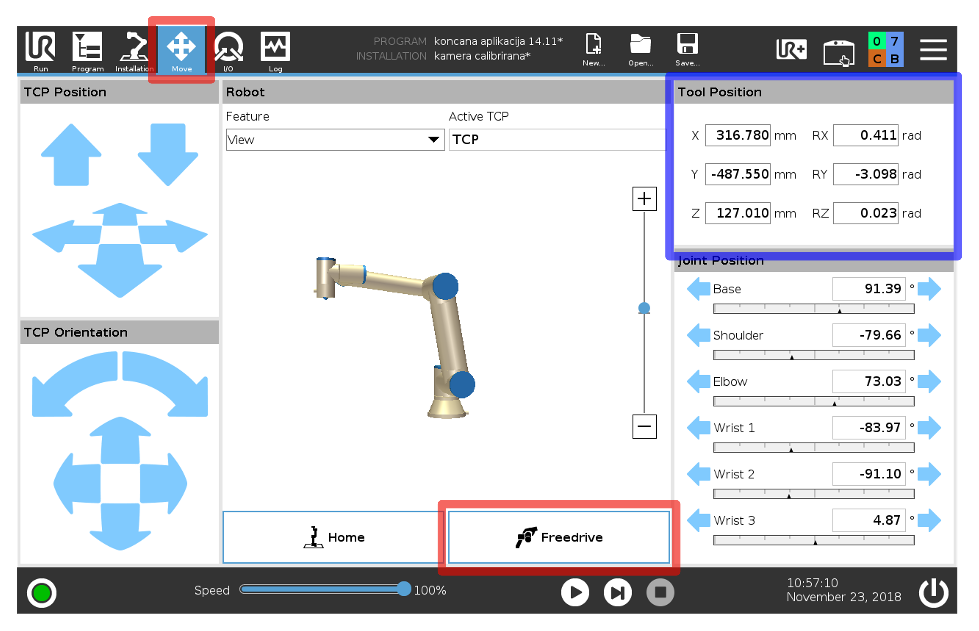
\includegraphics[width=0.6\columnwidth]{GUI_1.eps}
%\includegraphics{Graphic2.png}
  \caption{\label{delovno_okolje} Delovno okolje UR5e robota.}
\end{figure}

Za vodenje robota in prikaz trenutne pozicije robota izberete meni \emph{Move} (na sliki \ref{delovno_okolje} je označen z rdečim kvadratom). Robota je mogoče premikati z modrimi puščicami v oknih \emph{TCP Position} in \emph{TCP Orientation}. Možno pa je robota premikati z ročnim premikanje robotskega mehanizma, pri čemer morate držati gumb \emph{Freehand}. V oknu \emph{Tool Position} je zapisana lega robota (na sliki \ref{delovno_okolje} je označen z modrim kvadratom). S klikom na eno od vrednosti \emph{XYZ} pozicije, se vam odpre novo okno, ki je prikazano na sliki \ref{GUI_UR53_2}. V tem oknu izberete pravilen zapis orientacije vrha robota. Z modrim okvirjem je prikazan meni za izbiro zapisa orientacije. Izberete zapis \emph{RPY} $\left[ ^\circ \right]$. V poljih \emph{TCP} obkroženih z zelenim okvirjem je podan zapis lege robota. V polju \emph{Joint Position} obkroženih z rumenim okvirjem je podan zapis kotov v sklepih robota.


\begin{figure}[h]
	\centering
	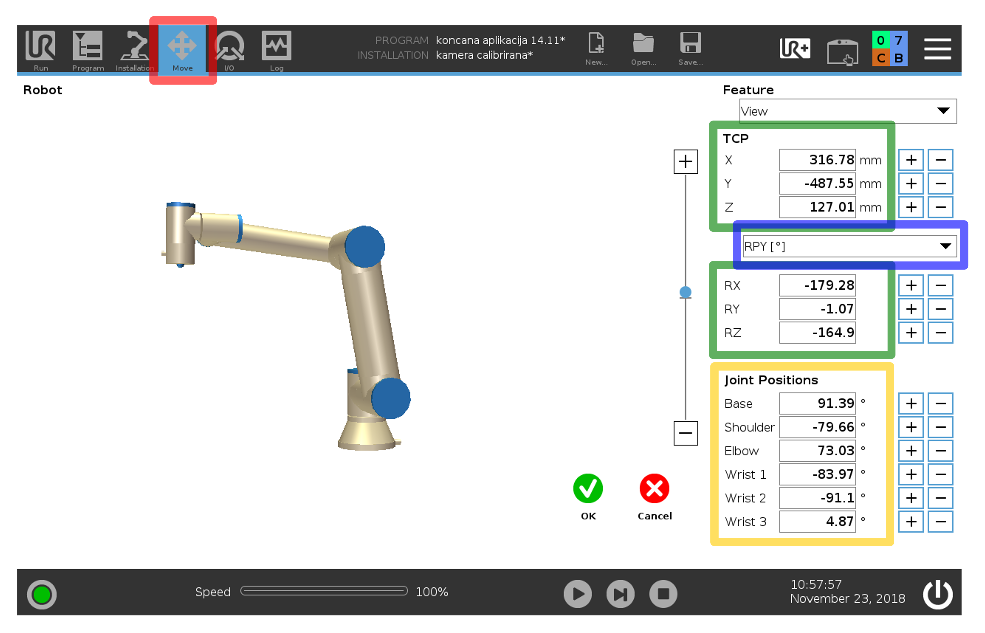
\includegraphics[width=0.6\columnwidth]{GUI_2.eps}
	%\includegraphics{Graphic2.png}
	\caption{\label{GUI_UR53_2} Okno za prikaz lege robota.}
\end{figure}

Preden primerjate vrednosti, ki ste jih izračunali samo z vrednostimi, ki jih podaja krmilnik, preverite, če imate izbrano pravo orodje. Slika \ref{GUI_UR53_3} prikazuje okno za izbor orodja pod menije \emph{Installation}. V polju \emph{Tool Center Point} je potrebno izbrati orodje prirobnice robota (na sliki je podan pod imenom \emph{TCP}).

\begin{figure}[h]
	\centering
	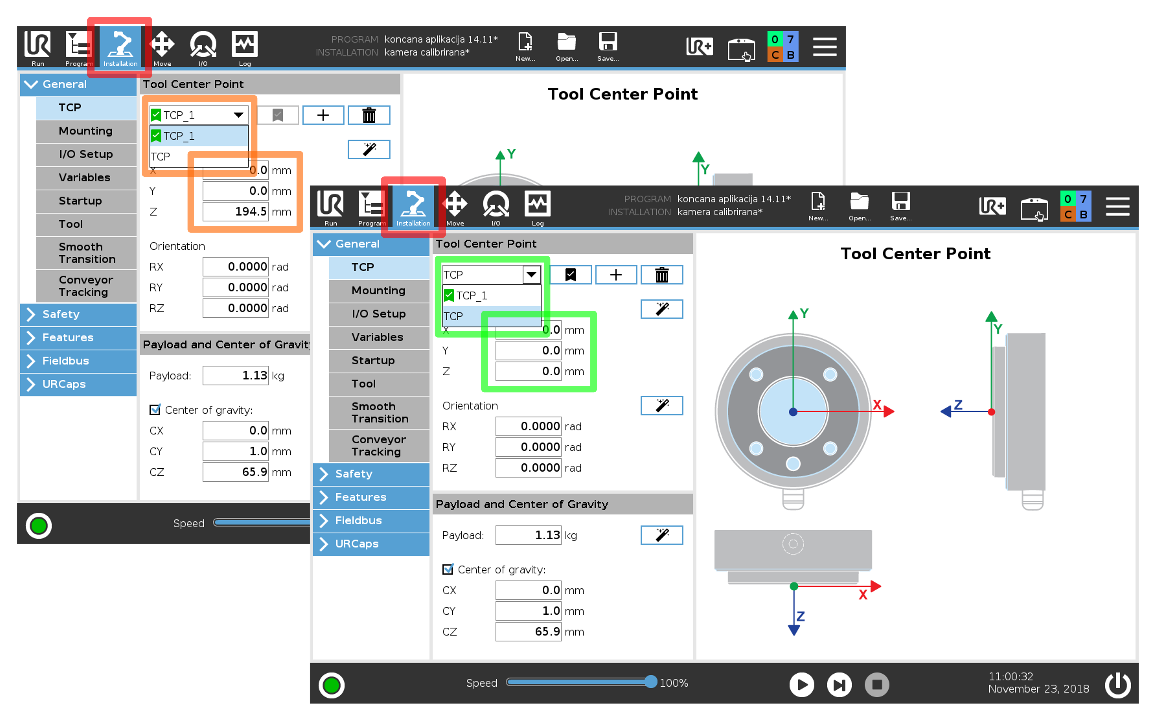
\includegraphics[width=0.6\columnwidth]{GUI_3.eps}
	%\includegraphics{Graphic2.png}
	\caption{\label{GUI_UR53_3} Okno za prikaz lege robota.}
\end{figure}

\subsection{Direktni kinematični model robota UR5e}

UR5e robot je robot antropomorfne konfiguracije s šestimi rotacijskimi sklepi. UR5e robot je sodelujoči robot in omogoča vodenje z roko. Na spletni povezavi https://www.universal-robots.com/academy/ je na voljo kratek tečaj za upravljanje z robotom. Robot je predstavljen na sliki \ref{fShemaUR5e}.

\begin{figure}[h]
    \centering
    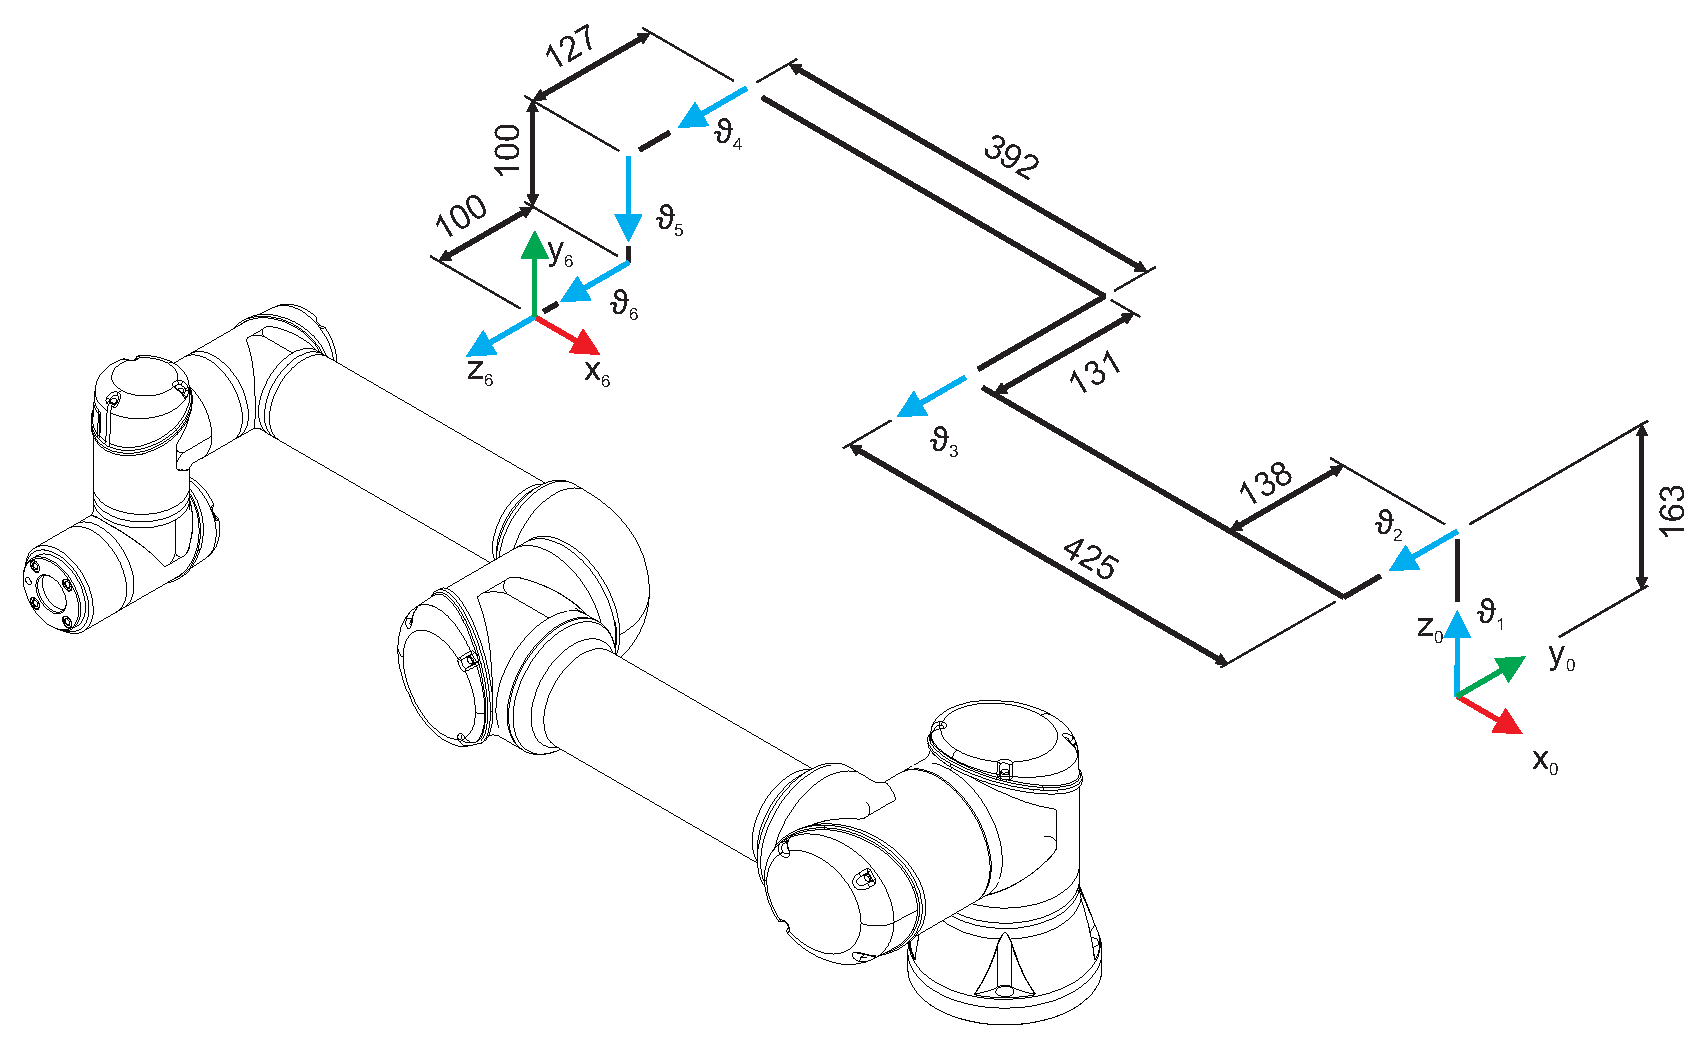
\includegraphics[width=0.85\textwidth]{UR5e_nicelna_lega.eps}
    \vspace{-0.3cm}
    \caption{Shema robota UR5e}
    \label{fShemaUR5e}
\end{figure}

\subsubsection{Metoda Denavit-Hartenberga}
Ob upoštevanju D-H pravil v sklepe robota postavite koordinatne sisteme.
Pomagajte si s sliko \ref{fShemaUR5e}. Določite D-H parametre, izračunajte
rotacijske matrike $A_i$ in podajte direktni kinematični model v analitični
obliki matrike $T_6$.

Izračunajte tudi numerično vrednost matrike $T_6$ za robota, ki bo postavljen v poljubni legi.

Numerično vrednost matrike $T_6$ določite na dva različna načina:
\begin{description}
  \item[Način 1] Matriko $T_6$ izračunajte s pomočjo zgoraj določenega kinematičnega modela robota.
  Podane so razdalje med posameznimi sklepi (glej sliko \ref{fShemaUR5e} ), vrednosti kotov v sklepih (notranje koordinate)
  pa odčitajte s programskega uporabniškega vmesnika za vodenje robota.
  \item[Način 2] Matriko $T_6$ izračunajte s pomočjo odčitane pozicije in orientacije vrha robota (zunanje koordinate).
  Podatke odčitate s programskega uporabniškega vmesnika za vodenje robota. Odčitajte tri podatke, ki opisujejo pozicijo vrha (x, y in z koordinato)
    in tri podatke, ki opisujejo rotacije vrha robota glede na referenčni K.S. (Rz - rotacija okrog $z$, Ry - rotacija okrog $y$ in Rx - rotacija okrog $x$ osi referenčnega K.S.).
\end{description}

Podatki o rotaciji vrha robota so zapisani v stopinjah. Za obdelavo v programu
\emph{Mathematica} jih moramo pretvoriti v radiane po enačbi: $\alpha =
\frac{\pi}{180^o} \alpha^o$. Informacijo o legi vrha pretvorimo v $T_6$
matriko po naslednji enačbi:
\begin{verbatim}
    T6 = Trans[{x,y,z}].RotZ[Rz].RotY[Ry].RotX[Rx]
\end{verbatim}
pri čemer: \newline \verb@Trans[{x,y,z}]@ vrne homogeno matriko
translacije za vektor, \newline \verb@RotX[Rx]@ vrne homogeno matriko
rotacije okrog $x$ osi referenčnega K.S. za kot $Rx$ v radianih,
\newline \verb@RotY[Ry]@ vrne homogeno matriko rotacije okrog $y$ osi
referenčnega K.S. za kot $Ry$ v radianih,
\newline \verb@RotZ[Rz]@ vrne homogeno matriko rotacije okrog $z$ osi
referenčnega K.S. za kot $Rz$ v radianih.

\subsubsection{Metoda vektorskih parametrov}

Spodaj je prikazana predloga Za$\_$studente$\_$UR5e.m za pisanje
vrstic programa za izračun direktnega geometrijskega modela za robot
UR5e. Vpisuje se samo vrstice, ki so označene s \emph{$\%$
STUDENT}. Vhodni parametri funkcije so: $th_1$, $th_2$, $th_3$, $th_4$, $th_5$ in $th_6$. Te
uporabite v kombinaciji s funkcijami za zapis homogenih
transformacijskih matrik.

\begin{figure}[h]
\scriptsize%
\textcolor[rgb]{0.13,0.55,0.13}{\textbf{\texttt{$\%$ ************************************}}}\\ %
\textcolor[rgb]{0.13,0.55,0.13}{\textbf{\texttt{$\%$ *** PREDLOGA ZA PISANJE PROGRAMA ***}}}\\ %
\textcolor[rgb]{0.13,0.55,0.13}{\textbf{\texttt{$\%$ ************************************}}}\\ %
\textcolor[rgb]{0.13,0.55,0.13}{\textbf{\texttt{$\%$ Programske vrstice vpisujete le v področja, ki so označena s STUDENT!}}}\\ %
\textcolor[rgb]{0.13,0.55,0.13}{\textbf{\texttt{$\%$ Ostale vrstice pustite nedotaknjene}}}\\ %
\textcolor[rgb]{0.13,0.55,0.13}{\textbf{\texttt{$\%$ *************************************************************************}}}\\ %
\textcolor[rgb]{0.00,0.00,0.00}{\textbf{\texttt{$\%$ function Za$\_$studente$\_$UR5e(th1,th2,th3,th4,th5,th6)}}}\\ %
\\ %
\textcolor[rgb]{0.13,0.55,0.13}{\textbf{\texttt{$\%$ *}}}\\ %
\textcolor[rgb]{0.13,0.55,0.13}{\textbf{\texttt{$\%$ **}}}\\ %
\textcolor[rgb]{0.13,0.55,0.13}{\textbf{\texttt{$\%$ ***}}}\\ %
\textcolor[rgb]{0.13,0.55,0.13}{\textbf{\texttt{$\%$ ***************************}}}\\ %
\textcolor[rgb]{0.13,0.55,0.13}{\textbf{\texttt{$\%$ *** VRSTICE ZA STUDENTE ***}}}\\ %
\textcolor[rgb]{0.13,0.55,0.13}{\textbf{\texttt{$\%$ *************************************************************************}}}\\ %
\textcolor[rgb]{0.13,0.55,0.13}{\textbf{\texttt{$\%$ th1 do th6 ... koti v sklepih v radianih}}}\\ %
\textcolor[rgb]{0.13,0.55,0.13}{\textbf{\texttt{$\%$ Definiranje homogenih transformacijskih matrik med sklepi}}}\\ %
\textbf{\texttt{\hspace*{1cm}H01 = \textcolor[rgb]{0.13,0.55,0.13}{$\%$ STUDENT}}}\\ %
\textbf{\texttt{\hspace*{1cm}H12 = \textcolor[rgb]{0.13,0.55,0.13}{$\%$ STUDENT}}}\\ %
\textbf{\texttt{\hspace*{1cm}H23 = \textcolor[rgb]{0.13,0.55,0.13}{$\%$ STUDENT}}}\\ %
\textbf{\texttt{\hspace*{1cm}H34 = \textcolor[rgb]{0.13,0.55,0.13}{$\%$ STUDENT}}}\\ %
\textbf{\texttt{\hspace*{1cm}H45 = \textcolor[rgb]{0.13,0.55,0.13}{$\%$ STUDENT}}}\\ %
\textbf{\texttt{\hspace*{1cm}H56 = \textcolor[rgb]{0.13,0.55,0.13}{$\%$ STUDENT}}}\\ %
\textbf{\texttt{\hspace*{1cm}H67 = \textcolor[rgb]{0.13,0.55,0.13}{$\%$ STUDENT}}}\\ %
\\ %
\textcolor[rgb]{0.13,0.55,0.13}{\textbf{\texttt{$\%$ Multiplikacija homogenih transformacijskih matrik za izračun}}}\\ %
\textcolor[rgb]{0.13,0.55,0.13}{\textbf{\texttt{$\%$ geometrijskega modela robota}}}\\ %
\textbf{\texttt{\hspace*{1cm}T = \textcolor[rgb]{0.13,0.55,0.13}{$\%$ STUDENT}}}\\ %
\textcolor[rgb]{0.13,0.55,0.13}{\textbf{\texttt{$\%$ *************************************************************************}}}\\ %
\textcolor[rgb]{0.13,0.55,0.13}{\textbf{\texttt{$\%$ ***}}}\\ %
\textcolor[rgb]{0.13,0.55,0.13}{\textbf{\texttt{$\%$ **}}}\\ %
\textcolor[rgb]{0.13,0.55,0.13}{\textbf{\texttt{$\%$ *}}}\\ %
\end{figure}
\vspace{-0.1cm} %

Ko zapišemo vse vrstice v obeh datotekah, zaženemo
uporabniško okno za preverjanje rezultatov. V ukazno vrstico programskega okolja Matlab vpišemo\\
\vspace{-0.2cm}\\%
\textbf{RezultatiGUI} \\ %
\vspace{-0.2cm}\\%
in odpre se okno s slike \ref{fGUI}.

\begin{figure}[h]
    \centering
    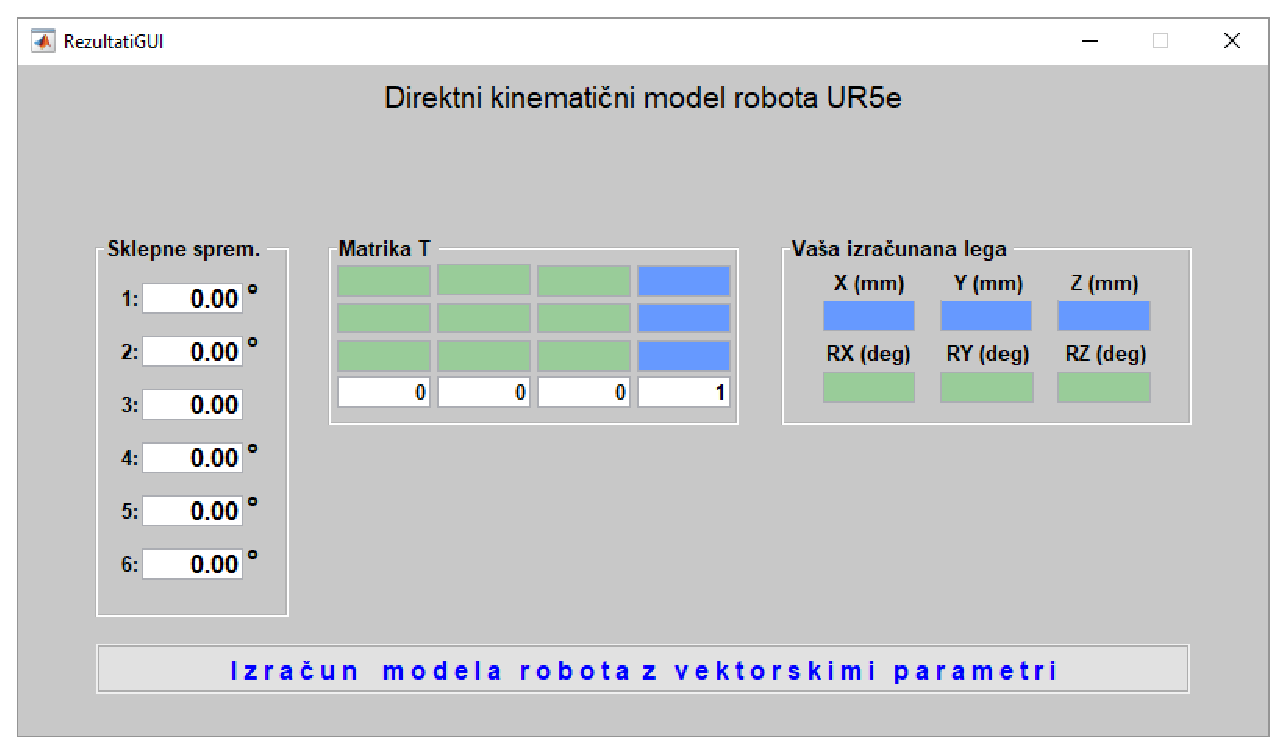
\includegraphics[width=0.74\textwidth]{matlab_vektorski_UR5e.eps}
    \vspace{-0.3cm}
    \caption{uporabniški vmesnik za preverjanje rezultatov}
    \label{fGUI}
\end{figure}

Objekti v uporabniškem vmesniku:

\begin{enumerate}
    \vspace{-0.2cm}%
    \item[] \textbf{Sklepne sprem.} $\longrightarrow$ Vpisujemo vrednosti sklepnih spremenljivk. %
    \vspace{-0.2cm}%
    \item[] \textbf{Matrika T} $\longrightarrow$ Transformacijska matrika vrha robota glede na ref. k.s. %
    \vspace{-0.2cm}%
    \item[] \textbf{Vaša izračunana lega} $\longrightarrow$ Pozicija in orientacija vrha glede na ref. k.s. %
    \vspace{-0.2cm}%
    \item[] \textbf{Izračun modela robota z vektorskimi parametri} $\longrightarrow$ Izračunamo kinematični model s svojimi parametri! %
\end{enumerate}



\subsection{Direktni kinematični model za robot Fanuc CR7i}

\subsubsection{Navodila za delo z ročno učno enoto robota Fanuc CR7i}

Na sliki \ref{delovno_okolje_CR7} je predstavljena ročna učna naprave robota Fanuc CR7i.
\begin{figure}[h]
\centering
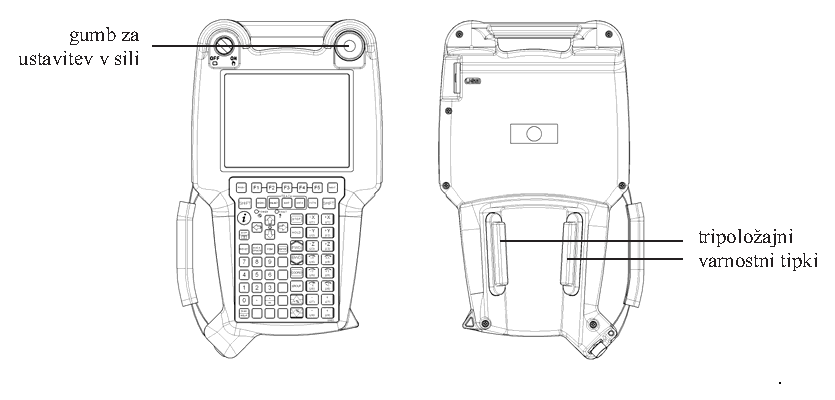
\includegraphics[width=0.6\columnwidth]{fanuc_teach_pendant.eps}
  \caption{\label{delovno_okolje_CR7} Ročna učna enota robota Fanuc CR7}
\end{figure}

Na sliki \ref{CR7_tipke} so označene pomembne tipke, ki jih boste potrebovali pri tej vaji.
\begin{figure}[h]
\centering
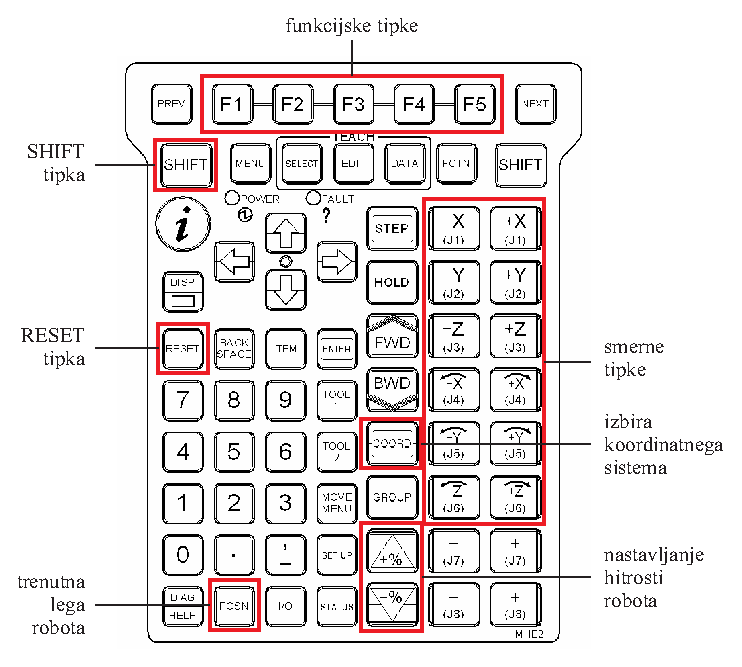
\includegraphics[width=0.6\columnwidth]{fanuc_tipke.eps}
  \caption{\label{CR7_tipke} Tipke na ročni učni napravi}
\end{figure}

Za vodenje robota je potreben sledeč postopek:
\begin{enumerate}
	\item pritisnite in držite levo ali desno tropoložajno varnostno tipko na zadnji strani ročne učne enote,
	\item pritisnite tipko \emph{RESET}
	\item spustite in še enkrat prisnite in držite tropoložajno varnostno tipko,
	\item pritisnite in držite tipko \emph{SHIFT},
	\item premikanje robota s smernimi tipkami na desni strani ročne učne naprave.
\end{enumerate}

Robota lahko premikate na več načinov: po posameznih sklepih (JOINT), premikanje vrha glede na osi baznega koordinatnega sistema (WORLD), glede na osi koordinatnega sistema vrha (TOOL) ali pa glede na osi uporabniškega koordinatnega sistema (USER).
Ustrezen koordinatni sistem izberete z večkratnim pritiskanjem na tipko \emph{COORD}. Kateri način je izbran, je prikazano v zgornji statusni vrstici (slika \ref{CR7_status}). Tu je vidna tudi trenutno izbrana hitrost premikanja robota; nastavljate jo lahko s tipkama \emph{$+$\%} in \emph{$-$\%}.

\begin{figure}[h]
\centering
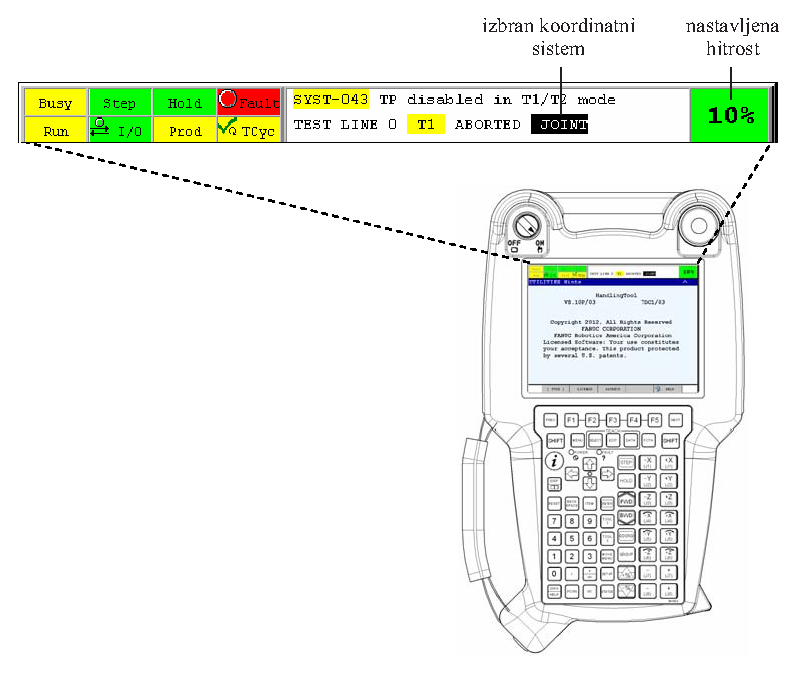
\includegraphics[width=0.6\columnwidth]{fanuc_status.eps}
  \caption{\label{CR7_status} Statusna vrstica}
\end{figure} 

Za prikaz trenutne lege robota pritisnite na tipko \emph{POSN} - druga tipka iz leve v spodnji vrstici. S funkcijskimi tipkami \emph{F2}, \emph{F3} in \emph{F4} izbirate med 
prikazom trenutnih vrednosti posamenih sklepov v stopinjah(JNT -- \emph{F2}}, trenutno lego vrha robota glede na uporabniški koordinatni sistem  (USER -- \emph{F3}) in trenutno lego vrha 
robota glede na bazni koordinatni sistem (WORLD -- \emph{F4}). Lega je opisana s tremi komponentami pozicije ($x$, $y$ in $z$) ter tremi koti v Roll-Pitch-Yaw (RPY) notaciji ($w$, $p$, $r$), kot je prikazan na sliki \ref{CR7_pos}.

\begin{figure}[h]
\centering
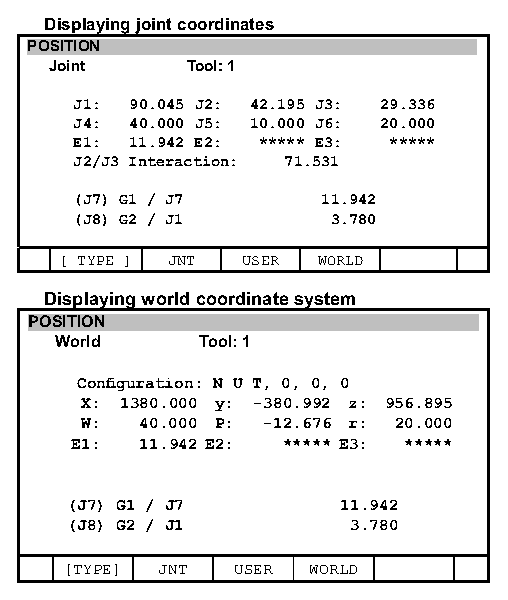
\includegraphics[width=0.5\columnwidth]{fanuc_pos.eps}
  \caption{\label{CR7_pos} Primer prikaza trenutne lege robota: po sklepih (zgoraj), glede na bazni koordinatni sistem (spodaj)}
\end{figure} 

Robota postavite v poljubno lego, nato pa na podlagi prebranih kotov v sklepih izračunajte direktni kinematični model robota po metodi Denavit-Hartenberg in po vektorski metodi. Dobljene rezulate primerjajte s podatki, ki so na voljo
preko ročne učne naprave (lega robota podana glede na bazni koordinatni sistem WORLD).

\subsection{Direktni kinematični model robota Fanuc CR7i}

Fanuc CR7i je robot antropomorfne konfiguracije s šestimi rotacijskimi sklepi. Sodelujoči robot ima v bazi integriran senzor sil in navorov, s katerim meri interakcijo z okolico. 
Robot je predstavljen na sliki \ref{fShemaCR7}.

\begin{figure}[h]
    \centering
    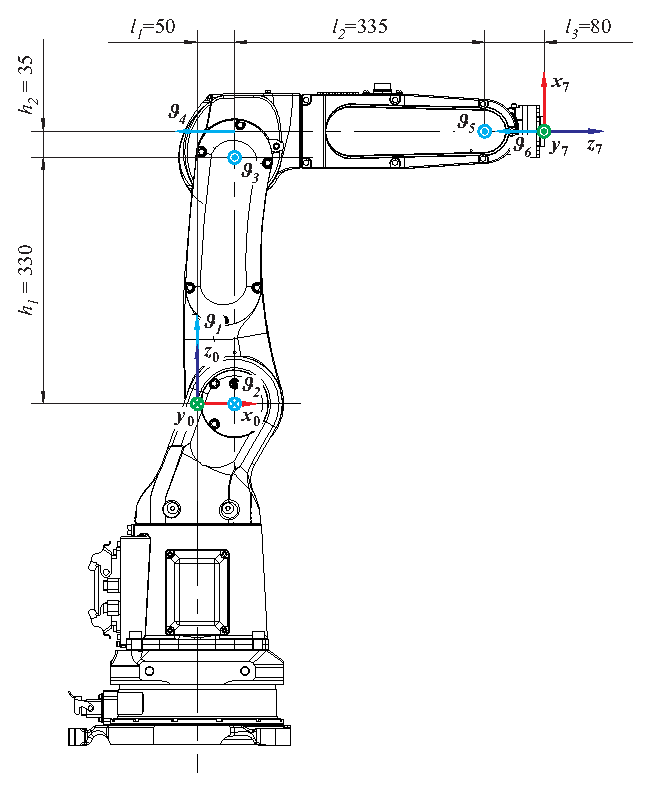
\includegraphics[width=0.7\textwidth]{fanuc_DH.eps}
    \vspace{-0.3cm}
    \caption{Shema robota Fanuc CR7i (s svetlo modro barvo so označene normale pozitivnih premikov posameznih osi)}
    \label{fShemaCR7}
\end{figure}

\subsubsection{Metoda Denavit-Hartenberga}
Ob upoštevanju D-H pravil v sklepe robota postavite koordinatne sisteme.
Pomagajte si s sliko \ref{fShemaCR7}. Določite D-H parametre, izračunajte
rotacijske matrike $A_i$ in podajte direktni kinematični model v analitični
obliki matrike $T_6$. Za izračun uporabite programski paket Mathematica.

Izračunajte tudi numerično vrednost matrike $T_6$ za robota, ki bo postavljen v poljubni legi.

Numerično vrednost matrike $T_6$ določite na dva različna načina:
\begin{description}
  \item[Način 1] Matriko $T_6$ izračunajte s pomočjo zgoraj določenega kinematičnega modela robota.
  Podane so razdalje med posameznimi sklepi (glej sliko \ref{fShemaCR7} ), vrednosti kotov v sklepih (notranje koordinate)
  pa odčitajte z ročne učne naprave. Pri tem bodize pozorni, da za tretji sklep (J3) privzamete vrednost \emph{J2/J3 Interlaced}.
  \item[Način 2] Matriko $T_6$ izračunajte s pomočjo odčitane pozicije in orientacije vrha robota (zunanje koordinate).
  Podatke odčitajte z ročne učne enote robota. Odčitajte tri podatke, ki opisujejo pozicijo vrha (x, y in z koordinato)
    in tri podatke, ki opisujejo rotacije vrha robota glede na referenčni koordinatni sistem. Orientacija je podana s tremi koti, zapisanimi v RPY notaciji (w - rotacija okrog $z$, p - rotacija okrog $y$ in r - rotacija okrog $x$ osi referenčnega koordinatnega sistema).
\end{description}

Podatki o rotaciji vrha robota so zapisani v stopinjah. Za obdelavo v programu
\emph{Mathematica} jih moramo pretvoriti v radiane po enačbi: $\alpha =
\frac{\pi}{180^o} \alpha^o$. Informacijo o legi vrha pretvorimo v $T_6$
matriko po naslednji enačbi:
\begin{verbatim}
    T6 = Trans[{x,y,z}].RotZ[w].RotY[p].RotX[r]
\end{verbatim}
pri čemer: \newline \verb@Trans[{x,y,z}]@ vrne homogeno matriko
translacije za vektor, \newline \verb@RotX[r]@ vrne homogeno matriko
rotacije okrog osi $x$ referenčnega koordinatnega sistema za kot $r$ v radianih,
\newline \verb@RotY[p]@ vrne homogeno matriko rotacije okrog osi $y$
referenčnega koordinatnega sistema za kot $p$ v radianih,
\newline \verb@RotZ[w]@ pa vrne homogeno matriko rotacije okrog osi $z$
referenčnega koordinatnega sistema za kot $w$ v radianih.

Dobljeni matriki primerjajte z lego vrha robota, podano glede na bazni koordinatni sistem, ki jo preberete na ročni učni napravi.

\subsubsection{Metoda vektorskih parametrov}

Ob upoštevanju pravil za metodo vektorskih parametrov označite na sliki koordinatne sisteme v sklepih, ustrezne smerne vektorje sklepov $\textbf{e}_i$, ter vektorje $\textbf{b}_{i-1,i}$, 
ki povezujejo izhodišča koordiantnih sistemov. Zapišite tudi ustrezne tabele sklepnih spremenljivk, vektorjev $\textbf{e}_i$ in vekorjev $\textbf{b}_{i-1,i}$. V programskem paketu Matlab izpolnite
predlogo za izračun direktnega geometrijskega modela za robota Fanuc CR7i. 

V nadaljevanju je prikazana Matlab predloga \verb@Za_studente_CR7.m@. Vpisuje se samo vrstice, ki so označene z \emph{$\%$
STUDENT}. Vhodni parametri funkcije so: $th_1$, $th_2$, $th_3$, $th_4$, $th_5$ in $th_6$. Te
uporabite v kombinaciji s funkcijami za zapis homogenih transformacijskih matrik.

\begin{figure}[h]
\scriptsize%
\textcolor[rgb]{0.13,0.55,0.13}{\textbf{\texttt{$\%$ ************************************}}}\\ %
\textcolor[rgb]{0.13,0.55,0.13}{\textbf{\texttt{$\%$ *** PREDLOGA ZA PISANJE PROGRAMA ***}}}\\ %
\textcolor[rgb]{0.13,0.55,0.13}{\textbf{\texttt{$\%$ ************************************}}}\\ %
\textcolor[rgb]{0.13,0.55,0.13}{\textbf{\texttt{$\%$ Programske vrstice vpisujete le v področja, ki so označena s STUDENT!}}}\\ %
\textcolor[rgb]{0.13,0.55,0.13}{\textbf{\texttt{$\%$ Ostale vrstice pustite nedotaknjene}}}\\ %
\textcolor[rgb]{0.13,0.55,0.13}{\textbf{\texttt{$\%$ *************************************************************************}}}\\ %
\textcolor[rgb]{0.00,0.00,0.00}{\textbf{\texttt{$\%$ function Za$\_$studente$\_$CR7(th1,th2,th3,th4,th5,th6)}}}\\ %
\\ %
\textcolor[rgb]{0.13,0.55,0.13}{\textbf{\texttt{$\%$ *}}}\\ %
\textcolor[rgb]{0.13,0.55,0.13}{\textbf{\texttt{$\%$ **}}}\\ %
\textcolor[rgb]{0.13,0.55,0.13}{\textbf{\texttt{$\%$ ***}}}\\ %
\textcolor[rgb]{0.13,0.55,0.13}{\textbf{\texttt{$\%$ ***************************}}}\\ %
\textcolor[rgb]{0.13,0.55,0.13}{\textbf{\texttt{$\%$ *** VRSTICE ZA STUDENTE ***}}}\\ %
\textcolor[rgb]{0.13,0.55,0.13}{\textbf{\texttt{$\%$ *************************************************************************}}}\\ %
\textcolor[rgb]{0.13,0.55,0.13}{\textbf{\texttt{$\%$ th1 do th6 ... koti v sklepih v radianih}}}\\ %
\textcolor[rgb]{0.13,0.55,0.13}{\textbf{\texttt{$\%$ Definiranje homogenih transformacijskih matrik med sklepi}}}\\ %
\textbf{\texttt{\hspace*{1cm}H01 = \textcolor[rgb]{0.13,0.55,0.13}{$\%$ STUDENT}}}\\ %
\textbf{\texttt{\hspace*{1cm}H12 = \textcolor[rgb]{0.13,0.55,0.13}{$\%$ STUDENT}}}\\ %
\textbf{\texttt{\hspace*{1cm}H23 = \textcolor[rgb]{0.13,0.55,0.13}{$\%$ STUDENT}}}\\ %
\textbf{\texttt{\hspace*{1cm}H34 = \textcolor[rgb]{0.13,0.55,0.13}{$\%$ STUDENT}}}\\ %
\textbf{\texttt{\hspace*{1cm}H45 = \textcolor[rgb]{0.13,0.55,0.13}{$\%$ STUDENT}}}\\ %
\textbf{\texttt{\hspace*{1cm}H56 = \textcolor[rgb]{0.13,0.55,0.13}{$\%$ STUDENT}}}\\ %
\textbf{\texttt{\hspace*{1cm}H67 = \textcolor[rgb]{0.13,0.55,0.13}{$\%$ STUDENT}}}\\ %
\\ %
\textcolor[rgb]{0.13,0.55,0.13}{\textbf{\texttt{$\%$ Multiplikacija homogenih transformacijskih matrik za izračun}}}\\ %
\textcolor[rgb]{0.13,0.55,0.13}{\textbf{\texttt{$\%$ geometrijskega modela robota}}}\\ %
\textbf{\texttt{\hspace*{1cm}T = \textcolor[rgb]{0.13,0.55,0.13}{$\%$ STUDENT}}}\\ %
\textcolor[rgb]{0.13,0.55,0.13}{\textbf{\texttt{$\%$ *************************************************************************}}}\\ %
\textcolor[rgb]{0.13,0.55,0.13}{\textbf{\texttt{$\%$ ***}}}\\ %
\textcolor[rgb]{0.13,0.55,0.13}{\textbf{\texttt{$\%$ **}}}\\ %
\textcolor[rgb]{0.13,0.55,0.13}{\textbf{\texttt{$\%$ *}}}\\ %
\end{figure}
\vspace{-0.1cm} %

Ko zapišemo vse vrstice v obeh datotekah, začenemo
uporabniško okno za preverjanje rezultatov. V ukazno vrstico programskega okolja Matlab vpišemo\\
\vspace{-0.2cm}\\%
\textbf{RezultatiGUI} \\ %
\vspace{-0.2cm}\\%
in odpre se okno s slike \ref{fGUI_CR7}.

\begin{figure}[h]
    \centering
    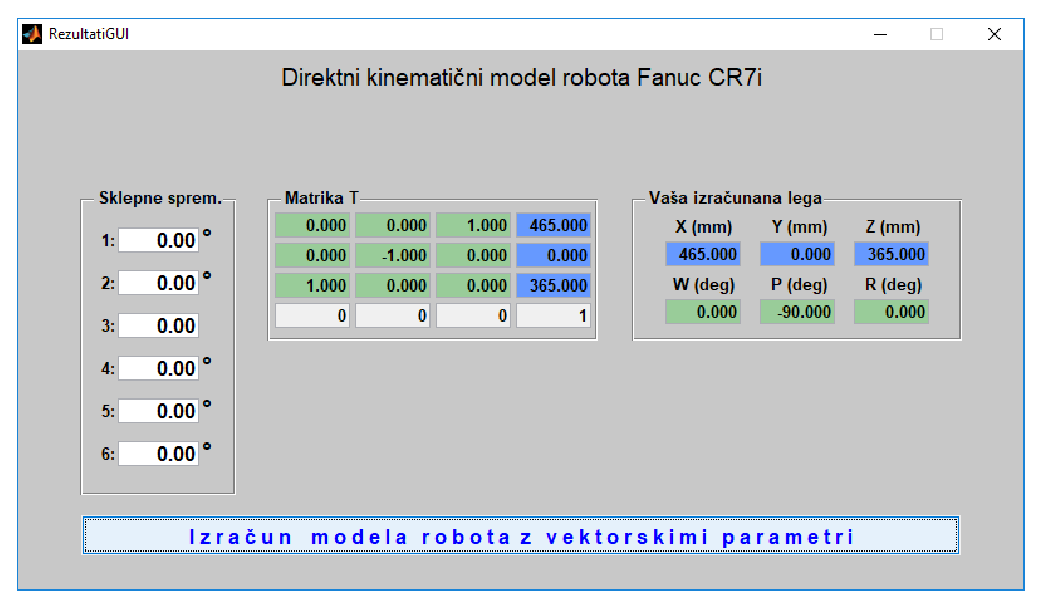
\includegraphics[width=0.74\textwidth]{fanuc_GUI.eps}
    \vspace{-0.3cm}
    \caption{Uporabniški vmesnik za preverjanje rezultatov - Fanuc CR7i}
    \label{fGUI_CR7}
\end{figure}

Objekti v uporabniškem vmesniku:
\begin{enumerate}
    \vspace{-0.2cm}%
    \item[] \textbf{Sklepne sprem.} $\longrightarrow$ Vpisujemo vrednosti sklepnih spremenljivk v stopinjah%
    \vspace{-0.2cm}%
    \item[] \textbf{Matrika T} $\longrightarrow$ Transformacijska matrika vrha robota glede na referenčni koordinatni sistem %
    \vspace{-0.2cm}%
    \item[] \textbf{Vaša izračunana lega} $\longrightarrow$ Pozicija in orientacija vrha glede na referenčni koordinatni sistem %
    \vspace{-0.2cm}%
    \item[] \textbf{Izračun modela robota z vektorskimi parametri} $\longrightarrow$ Poženemo izračun kinematičnega modela s svojimi parametri! %
\end{enumerate}

Na mesto sklepnih spremeljivk vpišite vrednosti kotov, ki ste jih prebrali na robotu v poljubni legi. Dobljen rezultat primerjajte z vrednostmi, ki jih prebrete na ročni učni napravi (lega vrha robota glede na bazni koordinatni sistem).